\documentclass[a4paper,12pt,leqno]{article}

\usepackage{natbib}
\usepackage{times}
\usepackage{url}
\usepackage{array}
\usepackage{latexsym}
\usepackage{caption}
\usepackage{amssymb,amsmath,amscd}
\usepackage{xcolor}
\usepackage[hang,flushmargin]{footmisc}
\usepackage{graphicx}  %%% for including graphics
\usepackage[margin=25mm]{geometry}
\usepackage{setspace}
\usepackage{diagbox}

\def\drs#1#2{
\begin{tabular}[c]{| c |}
	\hline #1 \\
	\hline #2 \\
	\hline
\end{tabular}
}

% Tim's custom commands
\newcommand{\bc}{{\rm b\!c}}
\newcommand{\unpad}{\mbox{{\rm unpad}}}
\newcommand{\vph}[1]{\vphantom{#1}}
\newcommand{\sta}[2]{\stackrel{#1}{#2}}


% David's custom commands
\newcommand{\ebox}[1]{\fbox{$\vph{'(),}#1$}}
\newcommand{\eboxl}[1]{\fbox{$\vph{'}#1$}}
\newcommand{\eboxh}[1]{\fbox{$\vph{,}#1$}}
\newcommand{\eboxb}[1]{\fbox{$\vph{@}#1$}}

\newcommand{\nbBefore}[2]{\ebox{#1}\ebox{}\ebox{#2}}
\newcommand{\nbMeets}[2]{\ebox{#1}\ebox{#2}}
\newcommand{\nbOverlaps}[2]{\ebox{#1}\ebox{#1,#2}\ebox{#2}}
\newcommand{\nbDuring}[2]{\ebox{#2}\ebox{#1,#2}\ebox{#2}}
\newcommand{\nbStarts}[2]{\ebox{#1,#2}\ebox{#2}}
\newcommand{\nbFinishes}[2]{\ebox{#2}\ebox{#1,#2}}
\newcommand{\nbEquals}[2]{\ebox{#1,#2}}

\newcommand{\nbAfter}[2]{\nbBefore{#2}{#1}}
\newcommand{\nbiMeets}[2]{\nbMeets{#2}{#1}}
\newcommand{\nbiOverlaps}[2]{\nbOverlaps{#2}{#1}}
\newcommand{\nbiDuring}[2]{\nbDuring{#2}{#1}}
\newcommand{\nbiStarts}[2]{\nbStarts{#2}{#1}}
\newcommand{\nbiFinishes}[2]{\nbFinishes{#2}{#1}}

\newcommand{\Before}[2]{\ebox{}\nbBefore{#1}{#2}\ebox{}}
\newcommand{\Meets}[2]{\ebox{}\nbMeets{#1}{#2}\ebox{}}
\newcommand{\Overlaps}[2]{\ebox{}\nbOverlaps{#1}{#2}\ebox{}}
\newcommand{\During}[2]{\ebox{}\nbDuring{#1}{#2}\ebox{}}
\newcommand{\Starts}[2]{\ebox{}\nbStarts{#1}{#2}\ebox{}}
\newcommand{\Finishes}[2]{\ebox{}\nbFinishes{#1}{#2}\ebox{}}
\newcommand{\Equals}[2]{\ebox{}\nbEquals{#1}{#2}\ebox{}}
\newcommand{\After}[2]{\ebox{}\nbAfter{#1}{#2}\ebox{}}
\newcommand{\iMeets}[2]{\ebox{}\nbiMeets{#1}{#2}\ebox{}}
\newcommand{\iOverlaps}[2]{\ebox{}\nbiOverlaps{#1}{#2}\ebox{}}
\newcommand{\iDuring}[2]{\ebox{}\nbiDuring{#1}{#2}\ebox{}}
\newcommand{\iStarts}[2]{\ebox{}\nbiStarts{#1}{#2}\ebox{}}
\newcommand{\iFinishes}[2]{\ebox{}\nbiFinishes{#1}{#2}\ebox{}}

\newcommand{\cBefore}[2]{``$#1$  before $#2$'' -- \Before{#1}{#2}}
\newcommand{\cMeets}[2]{``$#1$ meets $#2$'' -- \Meets{#1}{#2}}
\newcommand{\cOverlaps}[2]{``$#1$ overlaps $#2$'' -- \Overlaps{#1}{#2}}
\newcommand{\cDuring}[2]{``$#1$ during $#2$'' -- \During{#1}{#2}}
\newcommand{\cStarts}[2]{``$#1$ starts $#2$'' -- \Starts{#1}{#2}}
\newcommand{\cFinishes}[2]{``$#1$ finishes $#2$'' -- \Finishes{#1}{#2}}
\newcommand{\cEquals}[2]{``$#1$ equals $#2$'' -- \Equals{#1}{#2}}
\newcommand{\cAfter}[2]{``$#1$ after $#2$'' -- \After{#1}{#2}}
\newcommand{\ciMeets}[2]{``$#1$ imet by $#2$'' -- \iMeets{#1}{#2}}
\newcommand{\ciOverlaps}[2]{``$#1$ overlapped by $#2$'' -- \iOverlaps{#1}{#2}}
\newcommand{\ciDuring}[2]{``$#1$ contains $#2$'' -- \iDuring{#1}{#2}}
\newcommand{\ciStarts}[2]{``$#1$ started by $#2$'' -- \iStarts{#1}{#2}}
\newcommand{\ciFinishes}[2]{``$#1$ finished by $#2$'' -- \iFinishes{#1}{#2}}

\newcommand{\projects}[3]{\bc(\rho_{#3}(#1)) = #2}
\newcommand{\projectsVoc}[2]{\projects{#1}{#2}{voc(#2)}}

\renewcommand{\sp}{~\&~}
\newcommand{\spasync}{~\&_*~}
\newcommand{\spsigma}[1][\Sigma, \Sigma']{~\&_{#1}~}
\newcommand{\spvc}{~\&_{v\!c}~}

\renewcommand{\emptyset}{\varnothing}
\renewcommand{\phi}{\varphi}

% Allows entry of EventStrings as |a|{}|b,c|d|
% Use {} for empty box
\usepackage{etoolbox}
\DeclareListParser{\PipeParser}{|}
\newcommand{\EventString}[1]{
	\renewcommand*{\do}[1]{\ebox{##1}}%
	\PipeParser{#1}
}


\usepackage[nottoc,numbib]{tocbibind}

\doublespacing
%\linespread{2}


\title{\textbf{Strings for Temporal Annotation and\\Semantic Representation of Events}\\{\Large Theis in support of PhD}}

\author{\textbf{David Woods}\\
	ADAPT Centre\\
	Computational Linguistics Group\\
	School of Computer Science and Statistics\\
	Trinity College Dublin, Ireland\\
	\texttt{dwoods@tcd.ie}
}

\date{\parbox{\linewidth}{\centering%
		\today\endgraf\bigskip\bigskip\bigskip
		Supervised by: Tim Fernando, Carl Vogel}}

\begin{document}
\maketitle
\thispagestyle{empty}

\newpage
\pagenumbering{roman}
\begin{abstract}
\noindent
%This work describes the use of strings as models for the representation of temporal data -- i.e. events and times -- to form the basis of a framework for reasoning about that data. Some of the relevant motivating literature is examined, and a breakdown is given of the work done to develop and flesh out the framework so far, including discussion on superposition for collation of information into single, timeline-like strings, and projection which allows for the identification of temporal relations between arbitrary events and times from the strings. Possible ways of treating incomplete information are also looked at, including moving from intervals as primitives to semi-intervals. Some work done to implement this framework in code is described, with a discussion of potential applications in modern intelligent systems, including tooling for annotation software.
\end{abstract}

\newpage
\section*{Acknowledgements}
%My thanks to Tim for his patience and understanding, to Carl for guiding and reassuring comments, and to my friends and family for their continuous encouragement and support. In particular, Brian, who had the misfortune to be staying with me while I was working on this report, and the members of DU Trampoline club, who have had a more bad-tempered coach of late.

This research is supported by Science Foundation Ireland (SFI) through the CNGL 
Programme (Grant 12/CE/I2267) in the ADAPT Centre 
(\url{https://www.adaptcentre.ie}) at Trinity College Dublin. The
ADAPT Centre for Digital Content Technology is funded under the SFI Research 
Centres Programme (Grant 13/RC/2106) and is co-funded under the European 
Regional Development Fund.

\newpage
\section*{Publications}
%To date, I have had two papers accepted for publication: ``Towards Efficient String Processing of Annotated Events'' \citep*{woods2017towards}, which I presented at the 13th Joint ISO-ACL Workshop on Interoperable Semantic Annotation in Montpellier, France; and ``Improving String Processing for Temporal Relations'' \citep*{woods2018improving}, presented in Santa F\'{e}, New Mexico at the 14th Joint ISO-ACL Workshop on Interoperable Semantic Annotation, colocated with COLING 2018.

\newpage
\tableofcontents
\newpage
\pagenumbering{arabic}
%%%%%%%%%%%%%%%%%%%%%%%%%%%%%%%%%%%%%%%%%%%%%%%%%%%%%%%%%%%%%%%%%%%%%%%%%%%%%%%%
%                                                                              %
%                            Actual Document Begins                            %
%                                                                              %
%%%%%%%%%%%%%%%%%%%%%%%%%%%%%%%%%%%%%%%%%%%%%%%%%%%%%%%%%%%%%%%%%%%%%%%%%%%%%%%%
\section{Introduction}\label{sec:intro}
%The ability to reason about time and events is considered an essential aspect in several kinds of intelligent systems. For example, answering questions such as ``Which of our students were in receipt of a grant last year?" or ``How many conference papers were accepted last semester?" requires the use and interpretation of temporal information. Planning and scheduling systems rely on temporal reasoning in order to organise the data they process. Additionally, as human discourse and narrative often describes events out of chronological ordering, it's critical for natural language processing systems to be able to reason about sentences like ``Facebook's stock fell this morning after the controversy last night," so as to understand which event occurred first (the stock falling, or the controversy), in order for it to have an accurate understanding of the scenario.

%In order to perform reasoning about events and other time-related data in a useful way, it is first necessary to create a comprehensive framework for representing that temporal information in knowledge-based systems. Several approaches have been designed over the past years, based on a number of conventions and formalisms. The event calculus \citep{Kowalski1986,Miller1999,Mueller2008}, for example, represents events and their effects through the use of the predicates of a logical language. \citet{allen1983maintaining} used directed graphs to keep track of events and their inter-relations. T-BOX \citep{verhagen2005TBOX} draws semantically-placed boxes to similarly display the relations between events and times, using as its basis the TLINKs of TimeML \citep{Pustejovsky2005}, a markup language which has become an ISO standard for the annotation of text with explicit temporal data \citep{pustejovsky2010iso}.

%However, these frameworks do not offer a straightforward way to adequately and intuitively visualise a document's temporal structure without sacrificing the ability to perform efficient reasoning over that temporal information, and vice versa. For example, the formality of the event calculus is arguably not intuitive to a layperson, the directed graph approach of Allen suffers from a non-semantic layout, TimeML has no native graphical interface, and while T-BOX has an attractive design, it is not intended for use beyond being a visualisation aid (see Section \ref{sec:related} for more details on these tools). This work will describe a system which maintains both a compact visual appeal and a form which lends itself well to computation for logical inference and analysis.

%Using strings -- finite sequences of information $\alpha_1 \cdots \alpha_n$, $n \in \mathbb{N}$, where each $\alpha_i$ is a symbol representing some data -- is not uncommon for visualising the relations between events, evoking notions of Gantt charts and timelines. For example, these strings give a general picture of the relative order of two events X and Y:

%{
%\singlespacing
%\begin{center}
%\verb|XXX      |\\
%\verb|      YYY|\\
%\textit{``X occurs before Y occurs"}\\
%\vspace{1em}
%\verb|XXXXXXXXX|\\
%\verb|  YYYYY  |\\
%\textit{``Y occurs during X"}\\
%\end{center}
%}
%\noindent
%or see \citet[p. 835, Figure 2]{allen1983maintaining}, reproduced in Figure \ref{table:ARsorig} in Section \ref{sec:related}.
%
%The overarching question this work seeks to answer is {\sl How can strings be used to capture and represent temporal information in a precise and compact way for reasoning and processing, while evoking the intuition of timelines?} In order to tackle this, events and times must first be made representable as symbols in a simple and logical manner, so that they may be used as elements in a string. It is important that the strings may be used for semantic reasoning; that is, logical consequences may be inferred (for example, whether one set of temporal data entails another), allowing for useful deductions to be made. This work is also interested in ensuring that the framework be computationally tractable, so reducing algorithmic complexity and increasing data density are desirable. However, with this in mind, the intuitive presentational form of a timeline should be preserved where possible. The framework should be able to handle the complexities of real narratives to a satisfactory level, which may or may not contain complete data.
%
%Strings offer an excellent basis for this system which is to be created, as they are basic computational entities which are amenable to finite-state methods (such as decidably determining entailment of one string by another -- see Section \ref{sub:mso}), and reading them is intuitively similar to reading a timeline. The framework may have a number of applications in the field of intelligent systems, including among them annotation tooling. One of the hopes of this work is that it may be eventually implemented as a complementary tool for assisting with manual and semi-automatic annotation of temporal data in texts, alongside existant tools like T-BOX, which similarly strives for a semantic and intuitive presentation of temporal information.
%
%The rest of this text proceeds as follows: Section \ref{sec:related} below introduces the material which the current work uses as its foundation, including the interval-based framework for representing events/times and their inter-relations put forward by \citet{allen1983maintaining}, as well as TimeML (or more correctly, ISO-TimeML), which is an international standard for marking up texts with temporal annotations. Tango and T-BOX are also presented as similar attempts to provide a useful way of visualising temporal information for use in annotation environments. Section \ref{sec:current} goes into detail on the work completed so far towards answering the questions laid out above. The mechanics for using strings as a representational tool for temporality are described, as well as how one might compose multiple strings in order to increase data density. A number of operations are given that comprise the procedure for creation of the timeline-like structures, as well as operations which may be used for reasoning over them. Some issues are encountered relating to incomplete data and non-determinism, with an exploration of potential methods for handling such difficulties. Finally, Section \ref{sec:future} outlines what work remains to be done in solving the problems that have been set out here, as well as providing some thoughts on possible approaches to tackling the difficulties which arise.

%\newpage
%\section{Related Material}\label{sec:related}
%\subsection{Allen's Interval Algebra}\label{sub:allen}
%Much of the present work draws its roots in James F. \citeauthor{allen1983maintaining}'s work \textit{Maintaining Knowledge about Temporal Intervals} \citeyearpar{allen1983maintaining}. In this seminal paper, Allen described a framework for the use of temporal intervals (as opposed to points) as primitives to represent events and time periods. Many of the criteria he described as important in the design of his framework \citeyearpar[p. 833]{allen1983maintaining} remain valid and are implemented in the present work:
%\begin{enumerate}
%\onehalfspacing
%\item The representation should allow for the fact that much temporal information is relative rather than precise.
%\item Uncertainty of information should be allowed for, such as when the precise relation between two times is unknown (though constraints on the relation may exist).
%\item The granularity of reasoning should be flexible i.e. capable of dealing with years and seconds in the same manner.
%\item Reasoning should assume that states will persist unless there is some evidence to the contrary. In other words, \textit{change} is the marker of progression of time. 
%\end{enumerate}
%These principles guide Allen's temporal interval framework. Part of the motivation for using intervals rather than points is stated as follows:
%
%{
%\onehalfspacing
%\begin{quotation}
%\noindent
%``There seems to be a strong intuition that, given an event, we can always `turn up the magnification' and look at its structure. ... Since the only times we consider will be times of events, it appears that we can always decompose times into subparts. Thus the formal notion of a time point, which would not be decomposable, is not useful.'' \citep[p. 834]{allen1983maintaining}
%\end{quotation}
%}
%\noindent
%For example, an event \textit{Going-Home} could be broken down into sub-events \textit{Leaving-Work}, \textit{Commuting}, and \textit{Arriving-Home}, each of which could be further subdivided, repeatedly, as desired.
%
%Allen makes further argument for the use of intervals as primitive, disallowing zero-width time points, with an illuminating example involving a lightbulb being switched on: there must be an interval of time when the light was off, followed by an interval when it was on, but are these intervals open or closed? If they are open, then there is a time point between the two when the light is neither on nor off; however, if they are closed, then there is a time point when it is both on and off. This issue can be resolved by having the intervals be open at one end and closed at the other, although Allen calls this an artificial solution which ``emphasizes that a model of time based on points on the real line does not correspond to our intuitive notion of time'' \citeyearpar[p. 834]{allen1983maintaining}.
%
%However, this argument that temporal intervals are counter-intuitive if they are open on one end and closed at the other has not been universally accepted -- for example, event calculus \citep{Kowalski1986,Miller1999,Mueller2008} describes a predicate \textit{Initiates}$(e, f, t)$ which states that an event $e$ occurs at timepoint $t$, and the temporal proposition $f$ is true after $t$. In the lightbulb example, this is equivalent to using intervals which are open on the lower end and closed at the higher, which can be interpreted as meaning the light is not on at the initial moment of switching it on, but is afterwards.% We will return to this notion in our discussion of borders later {\color{red} reference the section}.

%Allen goes on to introduce the thirteen possible relations that can exist between two temporal intervals (including inverses):

%\begin{center}
%	\singlespacing
%	\begin{tabular}{| l l l l |}
%		\hline
%		\rule{0pt}{4ex}\textbf{Relation} & \textbf{Symbol} & \parbox[l]{60pt}{\textbf{Symbol for Inverse}} & \parbox[l]{60pt}{\textbf{Pictoral Example}} \\[10pt]
%		X \textit{before} Y & \textless & \textgreater & \verb|XXX YYY| \\[5pt]
%		X \textit{equal} Y & = & = & \verb|XXX| \\
%		& & & \verb|YYY| \\[5pt]
%		X \textit{meets} Y & m & mi & \verb|XXXYYY| \\[5pt]
%		X \textit{overlaps} Y & o & oi & \verb|XXX | \\
%		& & & \verb| YYY| \\[5pt]
%		X \textit{during} Y & d & di & \verb| XXX  | \\
%		& & & \verb|YYYYYY| \\[5pt]
%		X \textit{starts} Y & s & si & \verb|XXX  | \\
%		& & & \verb|YYYYY| \\[5pt]
%		X \textit{finishes} Y & f & fi & \verb|  XXX| \\
%		& & & \verb|YYYYY| \\[5pt]
%		\hline
%	\end{tabular}
%	\captionof{figure}{Allen interval relations \citep[p. 835, Figure 2]{allen1983maintaining}.}
%	\label{table:ARsorig}
%\end{center}
%These relations form part of the foundation of much of the present work, as they are fundamental in the specification of TimeML (to be introduced shortly), which provides the format for the corpus, TimeBank, which is currently being used to test the capabilities of the present system.

%The framework which Allen proposes is based on using a directed graph in which the nodes represent intervals, and the arcs are labelled according to the relation (or, in the case of uncertainty, relations) between the intervals. It is assumed that complete information about the relations in the network is maintained -- i.e. there are no nodes without an edge between them, as the transitivities between the various relations are computed as necessary, such as on the addition of a new interval into the network. For example, given a graph representing X \textit{before} Y (Fig. \ref{figure:simple-transitivity} (a)), a third node Z is added, with the information that Y is \textit{before} Z (Fig. \ref{figure:simple-transitivity} (b)). The relation between X and Z is then inferred using the fact that it has been constrained from thirteen possibilities to just one due to the transitivity rules which apply to the relations -- in this case X \textless{} Y and Y \textless{} Z results in X \textless{} Z (Fig. \ref{figure:simple-transitivity} (c)).
%\begin{center}
%	\begin{figure}[h]
%		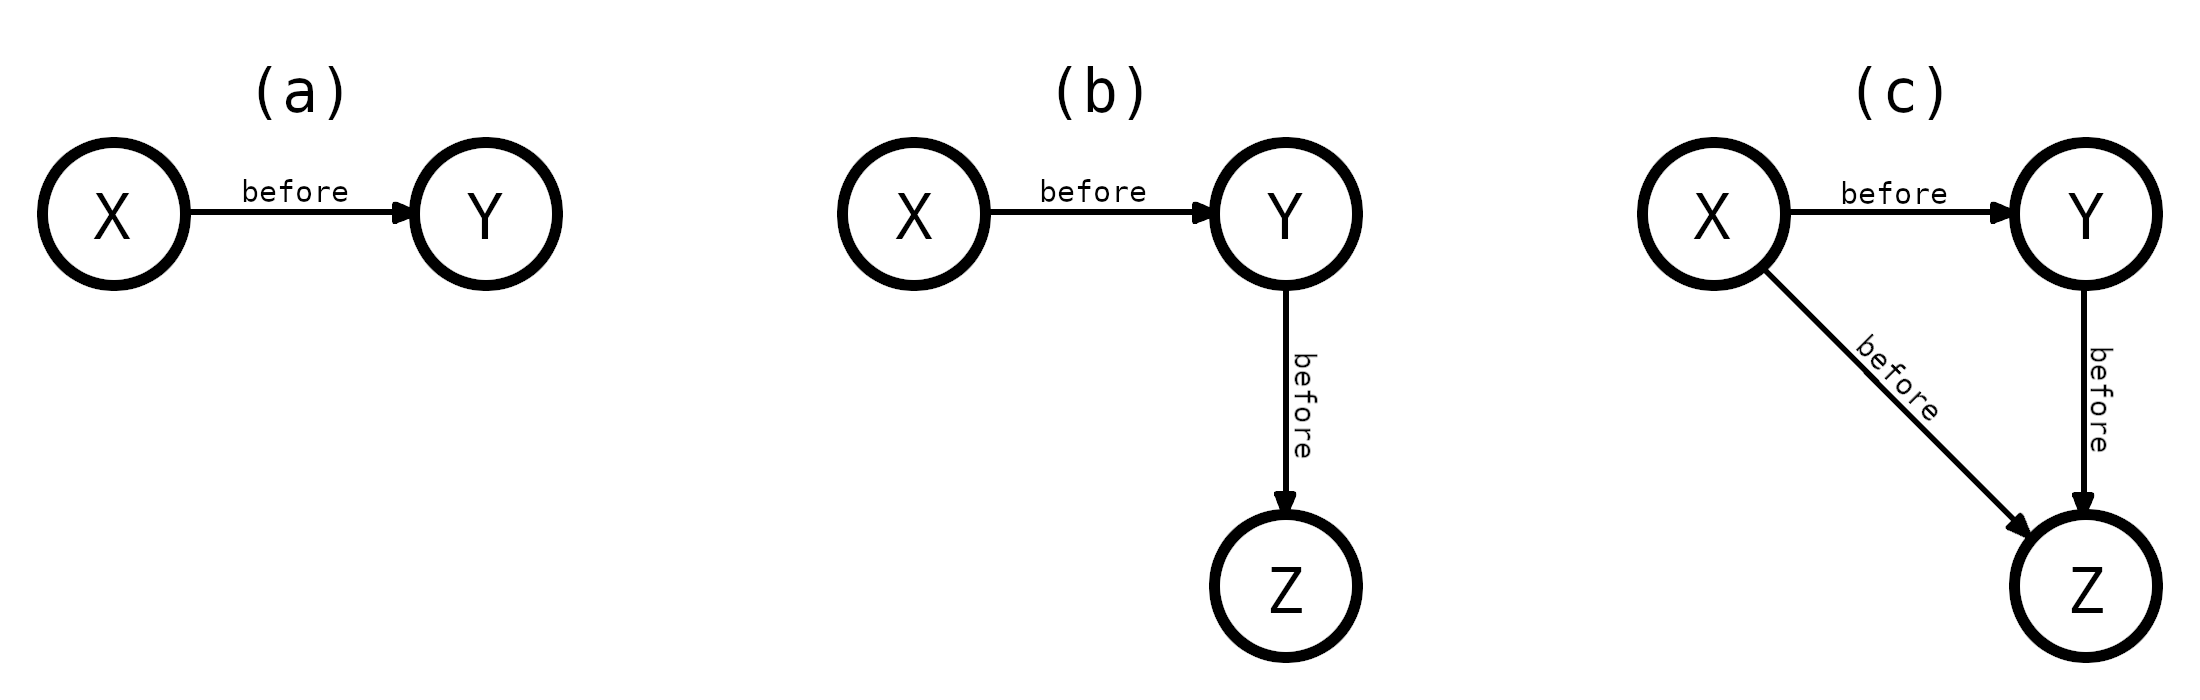
\includegraphics[width=\textwidth]{images/simple-transitivity}
%	\end{figure}
%	\captionof{figure}{Simple graph network showing the computation of a transitivity.}
%	\label{figure:simple-transitivity}
%\end{center}
%If there is a single label on every arc in the graph (of which there should be $N(N - 1)/2$ for $N$ nodes), then the complete \textit{temporal closure} has been calculated. This is a difficult (though desirable) goal given any real world data, as discourse often features incomplete or vague temporal information.\footnote{See \citet{Verhagen2005} for a discussion on temporal closure.}

%\citet[p. 836]{allen1983maintaining} also gives a $12 \times 12$ transitivity table (a fragment of which is reproduced below in Figure \ref{table:ttable}) which gives the possible relations between two intervals A and C, given the relations \textbf{r1} between A and B, and \textbf{r2} between B and C (omitting the ``equal" relation). A smaller fragment of this table is given in \citet[p. 130]{woods2017towards} showing these transitivities interpreted as superpositions of strings (see Section \ref{sec:current}). One immediate advantage of the string approach comes from the fact that the strings may describe the relations between more than three events at once.

%An algorithm is detailed \citep[p. 835]{allen1983maintaining} for the propogation of constraints upon the addition of new information to the network, using the transitivity table to update all arcs in the network as necessary. While Allen notes that there are some issues with the algorithm (specifically he mentions the space requirement, which is somewhat high at $O(N^2)$ space for $N$ temporal intervals, and the fact that the algorithm doesn't guarantee consistency in larger than three-node networks (something the current approach can do -- see Section \ref{sub:gentest}), and \citet[p. 219]{Verhagen2005} also notes an $O(N^3)$ time complexity), it does give an upper bound to the number of modifications that can be made to the network, regardless of the number of constraints added, as $13 \times \frac{(N - 1)(N - 2)}{2}$, and ``the average amount of work for each addition is essentially linear (i.e., $N$ additions take $O(N^2)$ time; one addition on average takes $O(N)$ time)" \citeyearpar[p. 837]{allen1983maintaining}. This is still quite high, given that it is not unusual for documents of the TimeBank corpus to feature fifty intervals or more, and some are in the hundreds \citep[p. 213]{Verhagen2005}.

%\begin{center}
%	\onehalfspacing
%	\begin{tabular}{|c|c|c|c|c|c|c|}
%		\hline
%		\diagbox{A \textbf{r1} B}{B \textbf{r2} C} & \textless{} & d & o & m & s & f\\
%		\hline
%		\textit{``before"} \textless{} & \textless{} & \textless{} o m d s & \textless{} & \textless{} & \textless{} & \textless{} o m d s\\
%		\hline
%		\textit{``during"} d & \textless{} & d & \textless{} o m d s & \textless{} & d & d\\
%		\hline
%		\textit{``overlaps"} o & \textless{} & o d s & \textless{} o m & \textless{} & o & o d s\\
%		\hline
%		\textit{``meets"} m & \textless{} & o d s & \textless{} & \textless{} & m & o d s\\
%		\hline
%		\textit{``starts"} s & \textless{} & d & \textless{} o m & \textless{} & s & d\\
%		\hline
%		\textit{``finishes"} f & \textless{} & d & o d s & m & d & f\\
%		\hline
%	\end{tabular}
%	\captionof{figure}{Fragment of Allen's transitivity table \citeyearpar[p. 836, Figure 4]{allen1983maintaining}.}
%	\label{table:ttable}
%\end{center}
%\cite[p. 838]{allen1983maintaining} also describes a method for grouping clusters of intervals which are fully computed in terms of the relations between them, termed ``reference intervals" due to the fact that each interval $I_i$ in the group $\{I_1, I_2, ..., I_n\}$ will reference some new interval $R_m$ (where $m$ is an index on the number of reference intervals). The motivation for these is to reduce the space requirements while maintaining as much of the inferential power as possible. Allen shows how, since these reference intervals are just treated as normal intervals, they may themselves be grouped into a cluster, and thus allow for the creation of hierarchies of intervals which may be useful for scenarios such as when a path search algorithm is to be used. These are not currently implemented in the present work, but they may be useful as a way to address documents with high numbers of intervals.

%Allen's work was and remains highly influential in the field as the approach is intuitive and straight-forward, as well as being easy to implement in various applications. One such proponent of interval relations has been TimeML, a markup language designed to ``capture the richness of temporal and event related information in language" \citep[p. 123]{Pustejovsky2005}.

%\subsection{TimeML}\label{sub:timeml}
%The initial motivation for creating the language lay in applications such as improving question answering systems by means of event recognition, and giving each event an explicit temporal location, due to the fact that a large proportion of temporal information in discourse (the domain primarily focused on by \citeauthor{Pustejovsky2005} is news articles) rely on implicit or vague temporal expressions. This relates to the first principle \citet{allen1983maintaining} mentioned as influencing his interval-based framework: that we do not intuitively think of or refer to time in terms of explicit/precise time points. Instead we tend to use relative expressions (e.g. ``I didn't go to work \textbf{last Monday}. I was sick \textbf{the week before}.") and rely on our listeners to be able to use context to interpret. Part of the goal with TimeML was to give implicit and relative temporal expressions an explicit anchoring, in order to assist with intelligent systems' temporal awareness. \citet{Pustejovsky2005} wanted to enable question answering systems to be able to answer questions such as (p. 125, (1a.)) ``Is Schr\"{o}der currently German chancellor?" as well as a human could after reading an appropriate news article. The authors raise a number of issues that ought to be addressed within a system that can understand and answer questions similar to this one. They also give several potentially problematic example queries, ranging from simple questions about the date of a specific event (e.g. ``When did Trinity first accept Catholic students?"), to questions about non-unique events (``How long does it take to drive to Cork?"), and questions where the system must perform some level of inference in order to derive the answer, possibly returning information that is not temporal in and of itself, but requires such data to find the correct solution (``Who was the last Taoiseach?").

%\citet[p. 245]{Pustejovsky2005} discuss the kinds of temporal information that might be needed, and how to go about representing it in a useful way. The authors state that two tasks are essential: the ability to place events on some timeline, and the ability to determine the relative order of any pair of events. These tasks are termed event \textit{anchoring} and \textit{ordering}, respectively, and these are also deemed a core part of the present work. Beyond these two tasks, the ability to identify and extract events and times from texts is an important task.

%Events are ``referred to by finite clauses, nonfinite clauses, nominalizations, event-referring nouns, adjectives, and even some kinds of adverbial clauses'' \citep[p. 246]{Pustejovsky2005}. Systems must also be aware of the possibility of negated and modal events, such as: ``Ireland did \textbf{not} \textit{make it} to the World Cup this year," and ``The exhibition \textbf{might} \textit{create} new opportunities for the museum.'' The events (italicised) in these sentences should not be treated as if they actually occurred. Additionally, care should be taken to distinguish separate events in the representation which are referred to together in the text: ``James \textit{taught 3 times} on Tuesday.'' \citep[p. 248, (32a.)]{Pustejovsky2005}.

%Times, on the other hand, generally take the form of adverbial or prepositional phrases in English, such as ``next week'', ``yesterday'', or ``10th of August''. The authors state that these expressions must be normalised in order to anchor events to times on a timeline -- normalising here means to convert them to some machine-readable form, possibly an integer or real number, depending on the context. It is also important to know the time of utterance (or document creation time, for a text) in order to correctly normalise expressions such as ``today'' or ``last Monday'', as these terms refer to a time relative to some other point (the time of utterance/document creation time). Some expressions, such as ``recently'' cannot be determinately linked to the timeline, due to their inherently vague nature -- however, they may still be ordered relative to other time points, and thus the normalisation process should have some method of handling them. The last two kinds of time expressions mentioned are durations (e.g. ``five hours'') which may or may not be anchored to times or events (``two years ago today'', ``a week before the match''), and sets of times, generally used to place recurring events on the timeline (e.g. ``every week'', ``twice a day'').

%While the current work deals directly with data that is already annotated with markers for events and times, it is worth keeping this instructive material on extraction of temporal data in mind. The TimeBank corpus \citep{pustejovsky2006timebank} is a large collection of documents (in the domain of news articles) manually annotated with TimeML, and as such contains a number of human errors (e.g. inconsistencies in relation-labelling). It is also not as completely labelled as it could be, and has also not been updated in several years. It is conceivable, then, that an alternative source for data may at some point become desirable, either due to the release of a more attractive corpus, or by creating an entirely new corpus, following the same general principles as in TimeBank.

%In order to perform ordering and anchoring, a set of relations for times and events is required. \citet[p. 235]{Pustejovsky2005} point to Allen's thirteen interval relations as a good basis for this, as reasoning over them is ``well-understood''. However, the authors note that not all of Allen's relations are equally well represented in the English language, suggesting that the \textit{overlaps} relation in particular is unnecessary. In fact they do omit this relation and its inverse from their final set, as shall be seen shortly.

%The syntax of TimeML uses four distinct types of tag to capture the various kinds of information: \verb|<TIMEX3>| for time expressions, \verb|<EVENT>| for events, \verb|<SIGNAL>| for functional words (e.g. \textit{at}, \textit{from}, etc.), and \verb|<LINK>| for relations between all of the other tags, subdivided into signal link \verb|<SLINK>|, aspectual link \verb|<ALINK>|, and temporal link \verb|<TLINK>|. The present work is most interested in this last tag type, as it is here that Allen's interval relations are represented, albeit under slightly different nomenclature (see Fig. \ref{table:TLINKs}). Each of TimeML's tags take a number of attributes which help to flesh out the representation of the information,\footnote{for the full specification of TimeML, see \url{http://www.timeml.org} \citep{timeml2005timeml}.} and for a TLINK these are: either a \texttt{timeID} or \texttt{eventInstanceID}, which refers to some temporal expression in the text; either a \texttt{relatedToTime} or \\\texttt{relatedToEventInstance}, which will refer to another temporal expression; and a \\\texttt{relType}, which will specify the relation from the first attribute to the second.
%\begin{center}
%	\onehalfspacing
%	\begin{tabular}{|c c|}
%		\hline
%		\textbf{TLINK} & \textbf{Allen}\\
%		\hline
%		\texttt{SIMULTANEOUS} & \textit{equal} =\\
%		\texttt{IDENTITY} & \textit{equal} =\\
%		\texttt{BEFORE} & \textit{before} \textless{}\\
%		\texttt{AFTER} & \textit{after} \textgreater{}\\
%		\texttt{IBEFORE} & \textit{meets} m\\
%		\texttt{IAFTER} & \textit{met by} mi\\
%		\texttt{INCLUDES} & \textit{contains} di\\
%		\texttt{IS\_INCLUDED} & \textit{during} d\\
%		\texttt{DURING} & \textit{during} d\\
%		\texttt{DURING\_INV} & \textit{contains} di\\
%		\texttt{BEGINS} & \textit{starts} s\\
%		\texttt{BEGUN\_BY} & \textit{started by} si\\
%		\texttt{ENDS} & \textit{finshes} f\\
%		\texttt{ENDED\_BY} & \textit{finished by} fi\\
%		\hline
%	\end{tabular}
%	\captionof{figure}{Possible values of a TLINK's relType attribute and their Allen relation counterparts.}
%	\label{table:TLINKs}
%\end{center}
%The rationale behind distinguishing \texttt{INCLUDES}/\texttt{IS\_INCLUDED} and \texttt{DURING\_INV}/\texttt{DURING} is that the former should be used for cases like ``He \textbf{arrived} there \textbf{last week},'' while the latter should be used specifically for states or events that persist throughout a duration, e.g. ``James was \textbf{CTO} for \textbf{two years}'' \citep[p. 273]{Pustejovsky2005}.

%Here is a simple example from the specification \citep[(11)]{timeml2005timeml}:
%``John taught 20 minutes every Monday.''

%{
%\singlespacing
%\verb|John|
%
%\verb|<EVENT eid="e1" class="OCCURRENCE">|
%
%\verb|taught|
%
%\verb|</EVENT>|
%
%\verb|<MAKEINSTANCE eiid="ei1" eventID="e1" pos="VERB" tense="PAST"|
%
%\verb|  aspect="NONE" polarity="POS"/>|
%
%\verb|<TIMEX3 tid="t1" type="DURATION" value="P20TM">|
%
%\verb|20 minutes|
%
%\verb|</TIMEX3>|
%
%\verb|<TIMEX3 tid="t2" type="SET" value="xxxx-wxx-1" quant="EVERY">|
%
%\verb|every Monday|
%
%\verb|</TIMEX3>|
%
%\verb|<TLINK timeID="t1" relatedToTime="t2" relType="IS_INCLUDED"/>|
%
%\verb|<TLINK eventInstanceID="ei1" relatedToTime="t1"|
%
%\verb|  relType="DURING"/>|
%
%}

%\noindent
%The TimeML language has enjoyed considerable success in terms of widespread adoption, thanks in some part at least to the release of a large corpus of (human) annotated documents known as TIMEBANK \citep{pustejovsky2003timebank}. Since the initial release of the specification in \citeyear{Pustejovsky2005}, TimeML has received numerous improvements and updates (although the core aspects remain the same), and has become and ISO standard for temporal annotation \citep{pustejovsky2010iso}. The corpus was also updated -- the current edition being TimeBank 1.2 -- in order to be in line with the updated specification \citep{pustejovsky2006timebank}. However, as a markup language for annotation, it does not come with any built-in way to visualise the information it describes, and so other tools have been created to try to help with this shortcoming.

%\subsection{Tango and T-BOX}\label{sub:otherrep}
%Manual annotation of temporal data in text is not a simple task \citep[pp. 213--214]{Verhagen2005}. As such, a number of tools have been designed with the aim of assisting an annotator in making more correct decisions, either by helping to visualise the temporal structure of the document, or by automatically computing relations or marking inconsistencies as the annotator works. For example, Tango \citep{pustejovsky2003tango} was developed with the aim of improving the annotation of documents with TimeML by allowing users to (literally) draw connections between times and events which were displayed graphically, as in Figure \ref{figure:tango}.
%\begin{center}
%	\begin{figure}[h]
%		\centering
%		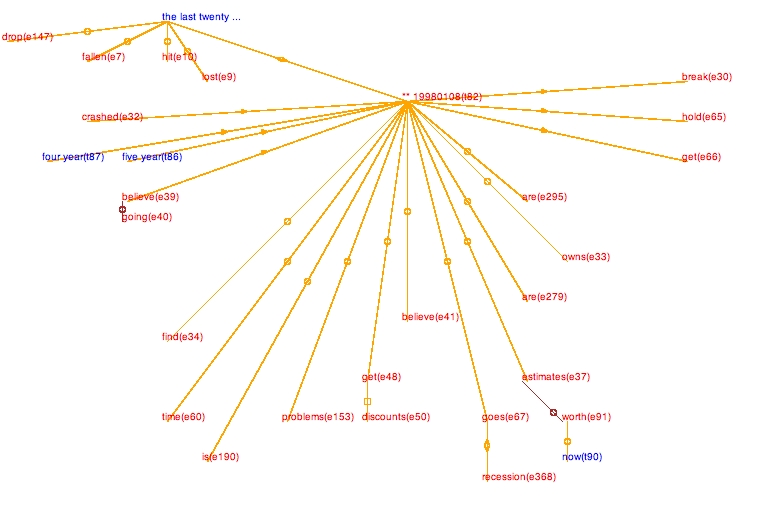
\includegraphics[width=0.85\textwidth]{images/tango}
%	\end{figure}
%	\captionof{figure}{Tango's interface \citep[taken from][p. 2, Fig. 1]{verhagen2005TBOX}.}
%	\label{figure:tango}
%\end{center}
%The graph here works on the same principle as those described in Section \ref{sub:allen}, in that the nodes represent the events and times which exist in the TimeML document, while the arcs are labelled with the relation between the intervals. According to \citet[p. 2]{verhagen2005TBOX}, using Tango improved the quality and reliability of the annotations being produced, with a higher number of links being found between the nodes, though he also notes that Tango's main flaw is that it does not allow a user to ``quickly capture the temporal structure of the document" \citep[p. 2]{verhagen2005TBOX} -- that is, interpreting the overall chronology of a text by means of a directed graph is not straightforward. Part of the problem, in \citeauthor{verhagen2005TBOX}'s opinion, is that the graph labels (representing the TLINKs of TimeML) are difficult to read, especially when the document contains a large number of nodes. More troublesome, however, is the fact that there is no inherent semantics to the placement of the nodes; there is no temporal ordering, left-to-right or otherwise, that is enforced by the system in a meaningful way.
%
%As a means of resolving some of these issues that he saw with Tango, \citet{verhagen2005TBOX} created the framework called T-BOX, which is based around the idea that ``relative placement of two events or times is completely determined by the temporal relations between them'' (p. 2). The image shown in Figure \ref{figure:tbox} represents the same data as in Figure \ref{figure:tango}, placing events and times in boxes, and using arrows, stacking, and box inclusion to represent the various relations between the temporal expressions.
%\begin{center}
%	\begin{figure}[h]
%		\centering
%		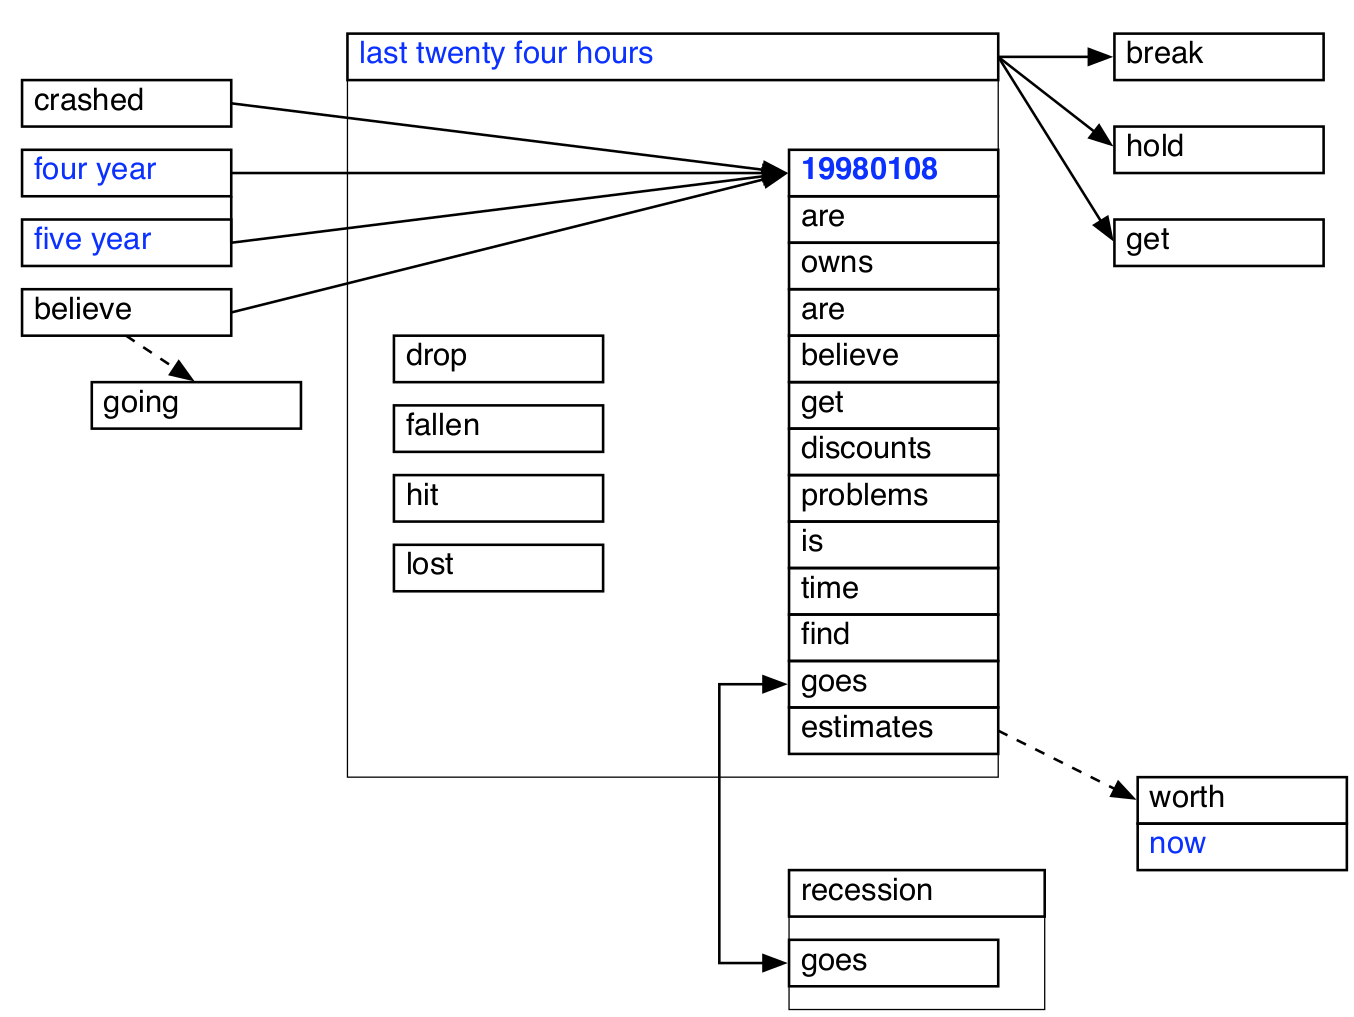
\includegraphics[width=0.7\textwidth]{images/tbox}
%	\end{figure}
%	\captionof{figure}{Fig. \ref{figure:tango}'s data now drawn using T-BOX \citep[taken from][p. 3, Fig. 2]{verhagen2005TBOX}.}
%	\label{figure:tbox}
%\end{center}
%The rules governing placement of boxes are \citep[pp. 3--5]{verhagen2005TBOX}:
%\begin{enumerate}
%\onehalfspacing
%\item An event which occurs \textit{before} another is placed to the left of it, with an arrow leading from one to the other, or a line ending in a dot if the relation is \textit{meets}.
%\item Simultaneous events are stacked, one box atop the other. Identical events are placed in the same box, rather than being treated the same as simultaneous ones.
%\item An event which \textit{contains} or \textit{includes} another gains an extended box with thinner walls, and the included event's box is placed inside this box.
%\item If an event \textit{starts} or \textit{finishes} another, it is placed inside that event's extended box, touching the left or right edge, respectively.
%\item Otherwise, none of these configurations may occur.
%\end{enumerate}
%\citeauthor{verhagen2005TBOX} stresses that the vertical and horizontal positioning of boxes doesn't mean anything in and of itself, and thus T-BOX abandons the ``timeline metaphor'' -- this is something which the present work intends to retain as far as possible.
%
%Another point of interest with T-BOX is that it requires as input a TimeML document which has complete temporal closure in its TLINKs, and then it reduces this to a minimal graph \citep[p. 6]{verhagen2005TBOX}. This is as opposed to the more typical scenario of trying to compute the temporal closure of a document using a constraint propogation algorithm (or, in the present case, the superposition of strings).
%
%A further benefit of the T-BOX is that it can be used to detect some inconsistencies in input data if there is some data which cannot be drawn using the rules given above. For example, if the TLINKs give that an event X is \textit{before} another event Y, that Y is \textit{before} a third event Z, and also that Z is \textit{before} X, the inconsistency will be discovered when attempting to draw X to the left of Y, which is to the left of Z, which should then somehow be drawn to the left of X. However, while non-drawability implies an inconsistency, drawability does not imply consistency \citep[p. 12]{verhagen2005TBOX}, since similarly to the constraint propogation algorithm in \citet{allen1983maintaining}, inconsistencies may appear in the graph which appear consistent when looking at three intervals, but become problematic in a larger context. Using strings avoids this issue, as inconsistent strings are ejected while performing superposition (see Section \ref{sub:gentest}).
%
%% \subsection{Finite State Approach to Temporality}
%% Tim stuff?
%
%\newpage
%\section{Work To Date}\label{sec:current}
%The present research explores alternative representational approaches for temporal information which may be used for reasoning and computation. Strings are used as models, due to the fact that they are basic computational entities, are amenable to finite-state methods, and have an intuitive similarity to timelines, as will be made clear below.
%
%The mechanics of how one may represent events and times within strings is described, as are a number of operations intended to maximise data density through the use of compression and superposition of multiple strings. Some preliminary work on the treatment of incomplete information using semi-intervals is also discussed, with the motivation of retaining the linearity of timelines, and avoiding non-determinism where possible. This proves to be challenging, although probabilistic methods may provide a solution (discussed in Section \ref{sub:incomplete}).
%
%\subsection{String Basics}\label{sub:basics}
%First, fix a finite set $A$ of \textit{fluents}, and encode sets of these fluents as symbols to allow any number of them to hold at once. A fluent $a \in A$ is understood here\footnote{Following the convention set out and used by \citet{Mccarthy69somephilosophical}, \citet{van2008proper}, and \citet{fernando2016prior}, among others.} to name a temporal proposition -- some event, state which may change (which will be referred to as an event, as in \citet{Pustejovsky2005}), or time period -- and the powerset $2^A$ of $A$ will serve as an alphabet for strings $s \in (2^A)^+$, which means that every string position will be a (possibly empty) set of fluents. For example, $A = \{js, fa, lt\}$, where $js = \text{``John sleeps"}$, $fa = \text{``A fire alarm is sounding''}$, and $lt = \text{``Last Tuesday"}$ -- these fluents might be used in modelling the sentence ``John slept through the fire alarm last Tuesday." Indeed, this can be done: \EventString{{}|lt|js,lt|fa,js,lt|js,lt|lt|{}} (an explanation follows below). It should here be noted that, for the time being, tense and aspect are abstracted away when using the string models. However, this can be remedied without too much strain using fluents to represent the speech and reference times, along with the event time \citep{fernando2016regular,Derczynski2013,reichenbach1947elements}.
%
%A string of $n$ sets $\alpha_1 \alpha_2 \cdots \alpha_n$ is used to represent a sequence of events and time periods such that the linear order and inter-relations of the events are clearly apparent, while unnecessary repetition of information is avoided. Such a string is interpreted such that the chronology is read from left to right, with each $\alpha_i \subset A$, $i \in \{1, 2, \ldots, n\}$, depicting one of $n$ moments in time like a snapshot, and specifying the set of exactly those temporal propositions, or fluents, which hold simultaneously (as unary predicates) at that moment $i$. A fluent $a \in \alpha_i$ is understood to be occurring before another fluent $a' \in \alpha_j$ iff $i < j$ and $a' \notin \alpha_i$. If $a \in \alpha_i$ and $a' \in \alpha_i$, then $a$ and $a'$ are occurring at the same time.
%
%Following the principles outlined in \citet{allen1983maintaining}, these strings model inertial worlds, whereby states persist unless changed. This notion is also found in event calulus \citep{Kowalski1986,Miller1999,Mueller2008}, and is known by the name \textit{commonsense law of inertia} \citep[p. 19]{shanahan1997solving}, and even Aristotle seems to have pointed to inertia as a default state: ``But neither does time exist without change'' (in \textit{Physics IV})\citeyear{aristotlePhysicsIV}. As a result of this, and the fact that each string position $\alpha_i$ is explicit as to whether a fluent $a$ holds at that moment ($a \in \alpha_i$) or not ($a \notin \alpha_i$), the frame problem is avoided (see \citet[pp. 30--31]{Mccarthy69somephilosophical}).\footnote{The frame problem is an issue that can arise in first-order logic representations of the world, whereby specifying the conditions which change as the result of an action is not sufficient to entail that no other conditions have changed.}
%
%The strings do not (necessarily) give any sense of duration. That is to say that the length of time represented by any $\alpha_i$ does not need to be equal to the length of time represented by any $\alpha_j$. Similarly, if a fluent $a$ appears in both $\alpha_i$ and $\alpha_{i+1}$, it is not understood as having a duration twice as long as if it had just appeared in $\alpha_i$. If $a$ appears in several string positions, the only thing affected is its relation to other fluents. Additionally, a string in which $\alpha_i = \alpha_{i+1}$ for any $1 \leq i < n$ will not have its interpretation affected if either $\alpha_i$ or $\alpha_{i+1}$ are deleted. For example, the string $\{a\}\{a\}\{a,b\}\{b\}\{b\}$ is equivalent in interpretation to $\{a\}\{a,b\}\{b\}$. A string featuring these repetitions is said to \textit{stutter}, and the process of removing stutter from a string is called \textit{block compression} \citep{fernando2015semantics,woods2017towards}, defined as follows:
%\begin{align}
%\onehalfspacing
%\bc(s) := 
%\begin{cases}
%	~~s & \text{if \textit{length}}(s) \leq 1\\
%	~~\bc(\alpha s') & \text{if } s = \alpha \alpha s'\\
%	~~\alpha \bc(\alpha' s') & \text{if } s = \alpha \alpha' s' \text{ with } \alpha \neq \alpha'
%\end{cases}
%\end{align}
%The inverse operation may also be used on \textit{stutterless} strings to generate infinitely many strings via the introduction of stutter:
%\begin{align}
%\onehalfspacing
%\bc^{-1}(\bc(s)) = \alpha_1^+ \alpha_2^+ \cdots \alpha_n^+ ~~~~~~~\mbox{ if } \bc(s) = \alpha_1 \alpha_2 \cdots \alpha_n
%\end{align}
%These strings are said to be \textit{\bc -equivalent} as they block compress to the same string. Precisely, strings $s$ and $s'$ are \bc -equivalent iff $\bc(s) = \bc(s')$. The usefulness of this will become apparent shortly.
%
%For convenience of notation, boxes are used instead of curly braces $\{\cdot\}$ to draw the sets which make up each string position (as in \citet{Fernando2004,fernando2015semantics,fernando2016prior}). This allows the strings to be read as if they were strips of film, or panels in a comic, creating the same narrative-style, intuitive feel as a timeline. An empty box \eboxb{} is drawn for the empty set $\emptyset$. This is a string of length 1, a moment of time during which none of the fluents we are looking at are holding. It should not to be confused with the empty string $\epsilon$, which has length 0, and contains no temporal information.
%
%For now, fluents are treated as intervals, as per \citet{allen1983maintaining}, and it shall also be assumed that each interval is bounded -- that is, there is time before and after $a$ holds during which $a$ does not hold, represented through the use of bounding empty sets -- although the framework does not require this assumption: the bounded interval $a$, drawn as \EventString{{}|a|{}}, as opposed to the non-bounded interval $a'$, drawn as \ebox{a'}.
%
%\subsection{Strings as MSO Models}\label{sub:mso}
%
%A further feature of these strings is that they may also be interpeted as finite models of Monadic Second-Order Logic (MSO).\footnote{See \citet{Libkin2012} for a discussion of MSO, a restricted form of Second-Order Logic in which quantification is only permitted for unary predicates (sets).} The benefit of this will become clearer after an example: the following string will serve this purpose, with the string positions indicated underneath each box:
%\begin{alignat}{5}\label{eq:ex-estr}
%\onehalfspacing
%\EventString{{}}&\EventString{a}&\EventString{a,a'}&\EventString{a}&\EventString{{}}&\\[-0.7em]
%{\scriptstyle 1}\kern 0.1em&~\kern 0.15em{\scriptstyle 2}&{\scriptstyle 3}~~~~&~\kern 0.15em{\scriptstyle 4}&{\scriptstyle 5}\kern 0.1em&\notag
%\end{alignat}
%(which represents the Allen relation $a'$ \textit{during} $a$, see Figure \ref{table:ARs}). The intervals $a$ and $a'$ can be identified by the string positions in which each occurs \citep{fernando2016regular,Fernando2018}:
%\begin{align}
%\onehalfspacing
%P_a = \{2,3,4\} ~\text{ and }~ P_{a'} = \{3\}
%\end{align}
%where $P_a$ and $P_{a'}$ are predicates interpreted as subsets of of $\{1,2,3,4,5\}$, the set of all of the string positions in (\ref{eq:ex-estr}).
%
%Generally, for any string $s = \alpha_1 \cdots \alpha_n$ of length $n$, the set of string positions $[n]$ is defined as
%\begin{align}
%\onehalfspacing
%[n] := \{1, \ldots, n\}
%\end{align}
%and for each $a \in A$ the predicate
%\begin{align}
%\onehalfspacing
%P_a := \{i \in [n] ~|~ a \in \alpha_i\}
%\end{align}
%specifies the positions where $a$ occurs. The successor relation is now defined:
%\begin{align}
%\onehalfspacing
%S_n := \{(i, i+1) ~|~ i \in [n - 1]\}
%\end{align}
%and finally $s$ can be described as the MSO$_A$ model
%\begin{align}
%\onehalfspacing
%Mod(s) := \langle [n], S_n, \{P_a\}_{a \in A} \rangle
%\end{align}
%There is a theorem due to B\"{u}chi, Elgot, and Trakhthenbrot (see, for example, \citet[p.124, Theorem 7.21]{Libkin2012}) which states that sentences $\phi$ of MSO capture regular languages, i.e. MSO-definability is equivalent to regularity. As such, the regular languages over the set $2^A$ of subsets of $A$ are given as \citep{Fernando2018}:
%\begin{align}
%\onehalfspacing
%\{s \in (2^A)^+ ~|~ Mod(s) \models \phi\}
%\end{align}
%Regular languages have been shown to be equivalent to finite automata (known as Kleene's theorem \citep[p. 41]{yu1997regular}), and thus these strings are open to manipulation using finite-state methods (see \citet{fernando2016regular}). For example, entailment of one language by another is decideable, which is not the case for First-Order Logic. This translates to being able to determine whether one string includes or entails another, which is a powerful feature for determining the relations that appear in a particular string (see Section \ref{sub:projection}).
%
%\subsection{Superposition}\label{sub:superposition}
%It is in the superposition of multiple strings that their usefulness becomes more evident: the information from several strings is combined into one, increasing the data density without compromising on detail, i.e. no precision is lost in favour of compression. The core motivating idea is that a number of strings may be extracted from an annotated source text, such as the documents of TimeBank \citep{pustejovsky2006timebank}, and subsequently these strings are combined with the goal of building a single resulting string to act as the timeline-like descriptor of the document's temporal structure. If a particular narrative doesn't contain a deterministic timeline such that a single string can be found, these methods will highlight that, and some possibilities for handling these situations are described later in Sections \ref{sub:semiintervals} and \ref{sec:future}. A number of other operations are also detailed in Section \ref{sub:projection} below to allow for focusing in on a smaller subsection of the timeline, or determining the relations between the events and time periods within the text.
%
%A basic notion of \textit{superposition} $\sp$ \citep{Fernando2002,woods2017towards} for two strings $s = \alpha_1 \alpha_2 \cdots \alpha_n$ and $s' = \alpha'_1 \alpha'_2 \cdots \alpha'_n$ of equal length $n$, is just their componentwise union:
%\begin{align}
%\onehalfspacing
%\alpha_1 \alpha_2 \cdots \alpha_n \sp \alpha'_1 \alpha'_2 \cdots \alpha'_n ~:=~ (\alpha_1 \cup \alpha'_1) (\alpha_2 \cup \alpha'_2) \cdots (\alpha_n \cup \alpha'_n)
%\end{align}
%for example
%\begin{align}\label{ex:sp}
%\onehalfspacing
%\EventString{a|a'|a''} \sp \EventString{a|a|a'} = \EventString{a|a,a'|a',a''}
%\end{align}
%%(Note that this form of the operation ignores semantics). 
%This is extended to languages (sets of strings) $L$ and $L'$ by simply collecting the superpositions of the strings of equal length in each language:
%\begin{align}
%\onehalfspacing
%L \sp L' ~:=~ \bigcup_{n\geq 0} \{s \sp s' ~|~ s\in L_n, ~s'\in L'_n\}
%\end{align}
%where $L_n$ and $L'_n$ are the sets of strings of length $n$ in $L$ and $L'$, respectively.
%
%Languages allow for some level of representation of non-determinism. Effectively, each string within a single language is an equally possible timeline. For example, suppose some ambiguity was introduced to (\ref{ex:sp}):
%\begin{align}\label{ex:splang}
%\onehalfspacing
%\{\EventString{a|a'|a''}, \EventString{a|a''|a'}\} \sp \{\EventString{a|a|a'}\} = \{\EventString{a|a,a'|a',a''}, \EventString{a|a,a''|a'}\}
%\end{align}
%The first input is a language containing two strings, either of which may be veridical (relative to whatever source data the strings are supposed to be representing). The resulting language also contains two strings -- it cannot be said which of these two is deterministically the ``correct" timeline, due to the ambiguity in the input. Languages containing a single string (as with the second input) can be conflated with that string, as it represents a deterministic timeline. One of the aims of this work is to reduce languages to small, finite sets, and ideally to singletons, so non-determinism is reduced.
%
%From the fact that strings are models of MSO, it may happen that these languages (depending on their source) be representable as regular languages. If $L$ and $L'$ are regular, accepted by finite automata $\langle Q, (2^A)^+, (q \sta{\alpha}{\to} r), q_0, F \rangle$ and $\langle Q', (2^{A'})^+, (q' \sta{\alpha'}{\to'} r'), q'_0, F' \rangle$, respectively, then $L \sp L'$ is also a regular language. It is computed by a finite automaton which is composed of the finite automata accepting $L$  and $L'$: $L \sp L'$ $\langle Q \times Q', (2^{A \cup A'})^+, ((q, q') \sta{\alpha \cup \alpha'}{\Rightarrow} (r, r')), (q_0, q'_0), F \times F' \rangle$ \citep{Fernando2004,woods2017towards}. %, where $Q$ and $Q'$ are the component state sets.
%
%Presently, the superposition operation prohibits combining strings of different lengths, which is desirable for allowing arbitrary numbers of fluents to appear in any one string. For example,
%\begin{align}\label{ex:spnoteqlen}
%\onehalfspacing
%\EventString{a|a'} \sp \EventString{a|a''|a'}
%\end{align}
%is not allowed as an operation, as it is not clear how to align the strings to perform the componentwise union. If each of these strings were in a language, and the languages were superposed, the result is an empty set. 
%
%To move past this restrictive requirement, the fact that introducing (or removing) stutter to/from a string does not change the result of its interpretation is exploited. The inverse block compression operation mentioned in Section \ref{sub:basics} can be used to increase the length of a string until it is suitable for the basic superposition operation.
%
%\textit{Asynchronous superposition} $\spasync$ between two strings $s$ and $s'$ is defined as the language obtained by block compressing the results of superposing strings which are \bc -equivalent to $s$ and $s'$ (note that $\bc(s) = \bc(s') \iff s' \in \bc^{-1}\bc(s')$):
%\begin{align}\label{def:spbc}
%\onehalfspacing
%s \spasync s' ~:=~ \{\bc(s'') ~|~ s'' \in \bc^{-1}\bc(s) \sp \bc^{-1}\bc(s')\}
%\end{align}
%Now it is possible to approach the situation in (\ref{ex:spnoteqlen}):
%\begin{align}\label{ex:spasync}
%\onehalfspacing
%\EventString{a|a'} \spasync \EventString{a|a''|a'} = \{&\EventString{a|a,a''|a'}, \EventString{a|a,a''|a,a'|a'}, \EventString{a|a'',a'|a'},\\
%&\EventString{a|a,a''|a'',a'|a'}, \EventString{a|a,a'|a'',a'|a'}\}\notag
%\end{align}
%It should be noted that since the operation $\bc^{-1}$ maps to an infinite language, some limit is required for the purposes of being able to practically compute the result of asynchronous superposition, and to avoid generating large amounts of redundant information. In \citet[p. 127]{woods2017towards}, an upper bound is established for the maximum length of any string produced by asynchronous superposition as $n + n' - 1$, where $n$ and $n'$ are the lengths of the operand strings $s$ and $s'$, respectively. The operation $pad_k$ is also introduced, which performs inverse block compression on a string, but the language which is produced contains only those strings which are of length $k$. For example:
%\begin{align}
%\onehalfspacing
%pad_4(\EventString{a|a'}) = \{\EventString{a|a|a|a'}, \EventString{a|a|a'|a'}, \EventString{a|a'|a'|a'}\}
%\end{align}
%As a result, the definition of asynchronous superposition is updated using this limit as follows:
%\begin{align}\label{def:spasync}
%\onehalfspacing
%\text{\textit{For any strings }}s, s' \in (2^A)^+\text{\textit{ with nonzero lengths $n$ and $n'$, respectively}}\notag\\
%s \spasync s' ~:=~ \{\bc(s'') ~|~ s'' \in pad_{n+n'-1}(s) \sp pad_{n+n'-1}(s')\}
%\end{align}
%
%Another note which is salient here is that neither basic superposition $\sp$ or asynchronous superposition $\spasync$ are ``aware" of the nature of the information on which they operate. That is to say, they are entirely syntactical operations, which do not care to retain the semantic information associated with their inputs. For example, in (\ref{ex:sp}), both of the operand strings contain the relation $a$ \textit{meets} $a'$, but the result instead claims that $a$ \textit{overlaps} $a'$, and in (\ref{ex:spasync}), one might expect some sort of issue to arise, since the first operand has $a$ \textit{meets} $a'$, while the second contradicts it, saying $a$ \textit{before} $a'$, but in fact five strings are returned, three of which contain $a$ \textit{meets} $a'$ and two which have $a$ \textit{overlaps} $a'$. The next two sections aim to resolve this issue.
%
%\subsection{Projection to Allen's Relations}\label{sub:projection}
%A point of interest is that the thirteen interval relations given by Allen fall out of the asynchronous superposition of two bounded intervals:
%\begin{align}
%\onehalfspacing
%\EventString{{}|a|{}} \spasync \EventString{{}|a'|{}} = \{\mbox{$\cal{S}$}_R(a, a') ~|~ R \in \{<, >, \mbox{d, di, f, fi, m, mi, o, oi, s, si}, =\}\}
%\end{align}
%with each string $\mbox{$\cal{S}$}_R(a,a')$ featuring one relation $a ~R~ a'$, as shown in Figure \ref{table:ARs} (from \citet[p. 79, Table 1]{woods2018improving}).
%\begin{center}
%	\onehalfspacing
%	\begin{tabular}{c|c|c||c|c|c}
%		$R$ & $a~R~a'$ & $\mbox{$\cal{S}$}_R(a,a')$ & $R^{-1}$ & $a~R^{-1}~a'$ & $\mbox{$\cal{S}$}_{R^{-1}}(a,a')$ \\
%		\hline
%		$<$ & $a$ before $a'$ & \Before{a}{a'} & $>$ & $a$ after $a'$ & \After{a}{a'} \\
%		
%		m & $a$ meets $a'$ & \Meets{a}{a'} & mi & $a$ met by $a'$ & \iMeets{a}{a'} \\
%		
%		o & $a$ overlaps $a'$ & \Overlaps{a}{a'} & oi & $a$ overlapped by $a'$ & \iOverlaps{a}{a'} \\
%		
%		d & $a$ during $a'$ & \During{a}{a'} & di & $a$ contains $a'$ & \iDuring{a}{a'} \\
%		
%		s & $a$ starts $a'$ & \Starts{a}{a'} & si & $a$ started by $a'$ & \iStarts{a}{a'} \\
%		
%		f & $a$ finishes $a'$ & \Finishes{a}{a'} & fi & $a$ finished by $a'$ & \iFinishes{a}{a'} \\
%		
%		= & $a$ equals $a'$ & \Equals{a}{a'} & & &
%	\end{tabular}
%	\captionof{figure}{Allen interval relations in strings}
%	\label{table:ARs}
%\end{center}
%Some further useful notation and mechanics are now introduced. First, it will be said that the \textit{vocabulary} of a string $s$ is the union of each of its components:
%\begin{align}
%\onehalfspacing
%voc(s) := \bigcup_{i=1}^n \alpha_i
%\end{align}
%This gives the set of fluents which are present in that string $s$.
%
%Next, for any set $A$, the $A$\textit{-reduct} $\rho_A$ of a string $s$ is the componentwise intersection of $s$ with $A$ \citep{fernando2016regular,woods2018improving}:
%\begin{align}
%\onehalfspacing
%\rho_A(\alpha_1 \alpha_2 \cdots \alpha_n) ~:=~ (\alpha_1 \cap A) (\alpha_2 \cap A) \cdots (\alpha_n \cap A)
%\end{align}
%This operation allows for control over exactly which temporal information of interest from a string will appear in it. For example, one may want to focus on the temporal relation between two fluents $a$ and $a'$, but have a string with far more data in it, so a $\{a, a'\}$-reduct is performed to remove the information which we are not concerned with:
%\begin{align}
%\onehalfspacing
%\rho_{\{a, a'\}}(\EventString{{}|a,x|a,x,y|a,y,a'|a,z|z|{}}) = \EventString{{}|a|a|a,a'|a|{}|{}}
%\end{align}
%Proceeding one step further, and block compressing the result of the reduct, the result is
%\begin{align}
%\onehalfspacing
%\bc(\EventString{{}|a|a|a,a'|a|{}|{}}) = \During{a'}{a}
%\end{align}
%which can be compared to the strings in Figure \ref{table:ARs} to determine that, in this example, $a'$ was during $a$.
%
%In order to streamline this process, it will next be said that a string $s$ \textit{projects to} another string $s'$ if the $voc(s')$-reduct of $s$ block compresses to $s'$ \citep{woods2018improving}:
%\begin{align}
%\onehalfspacing
%\projectsVoc{s}{s'}
%\end{align}
%Now, taking any string $s$ and pair of fluents $a$ and $a'$, their relation within $s$ can be determined by seeing which string in $\mbox{$\cal{S}$}_R(a,a')$ $s$ projects to. As a model of MSO, it can also be said that a string $s$ \textit{satisfies} or \textit{entails} $a ~R~ a'$ ($a ~R~ a'$ is true in $s$) if $s$ projects to $\mbox{$\cal{S}$}_R(a,a')$:
%\begin{align}
%\onehalfspacing
%s \models a ~R~ a' \iff \projects{s}{\mbox{$\cal{S}$}_R(a,a')}{\{a,a'\}}
%\end{align}
%Note that a language $L$ can also be said to project to a string $s'$ if every string $s \in L$ projects to $s'$, and a string projects to itself if and only if it is stutterless \citep{woods2018improving}.
%
%This described notion of projection is particularly useful, as it allows one to very quickly perform temporal reasoning, extracting and identifying the relations between various temporal expressions. By using the combination of reduction and compression, the operational granularity may be effectively controlled. Projection will also be used to further improve the superposition operation.
%
%\subsection{Generation While Testing}\label{sub:gentest}
%The key idea here is that a string in $s \spasync s'$ that is the result of the asynchronous superposition of $s$ and $s'$ should be able to project back to both $s$ and $s'$. If it cannot, then some part of the data has become lost or ``corrupted". Provided the vocabularies of the two strings are disjoint (i.e. $voc(s) \cap voc(s') = \emptyset$), then there is in general no issue. However, if this is not the case, as in the scenario when trying to combine information from two strings which feature the same fluent, then superposition as it is currently defined need not preserve the projections. For example:
%\begin{align}\label{ex:noproj}
%\Before{a}{a'} \spasync \Before{a'}{a''} = \{&\EventString{{}|a,a'|{}|a',a''|{}},\EventString{{}|a'|a,a'|{}|a',a''|{}},\EventString{{}|a'|a|{}|a',a''|{}},\\
%&\EventString{{}|a'|a|a''|a',a''|{}},\EventString{{}|a'|a|a''|a'|{}}, \ldots\}\notag
%\end{align}
%This result language contains 270 strings, and in fact, only one of these will in fact project back to both of the input strings: namely \EventString{{}|a|{}|a'|{}|a''|{}}.
%
%In \citet{woods2017towards}, the approach taken was to perform asynchronous superposition, and test the generated strings (using an algorithm based on matching string positions of padded input strings) to ensure that only correct strings were finally produced. However, while this does give the desired results, it is rather inefficient. In (\ref{ex:noproj}), 269 of the generated strings must be discarded. While simply altering the testing algorithm to use projection rather than using the string position matching method would already be a small improvement, in \citet{woods2018improving}, a new version of superposition was defined, called \textit{vocabulary constrained superposition} $\spvc$, which integrates projection-based testing into the generation process, meaning problematic strings are prevented from being produced at all. The definition is below.
%
%Begin by fixing an infinite set of fluents $\Theta$, and $Fin(\Theta)$ as the set of finite subsets of $\Theta$, such that for any string $s$, $s \in Fin(\Theta)^*$. Given $\Sigma, \Sigma' \in Fin(\Theta)$, a function $\&_{\Sigma,\Sigma'}$ is defined:
%\begin{align}
%\onehalfspacing
%\&_{\Sigma,\Sigma'} : (Fin(\Theta)^* \times Fin(\Theta)^*) \to 2^{Fin(\Theta)^*}
%\end{align}
%which maps a pair of strings $(s,s')$ to a set of strings $s \spsigma s' \subseteq Fin(\Theta)^*$ as follows:
%\begin{align}
%\onehalfspacing
%\epsilon \spsigma \epsilon ~:=~ \{\epsilon\}
%\end{align}
%where $\epsilon$ is the empty string (of length 0)
%\begin{subequations}
%\begin{align}
%\onehalfspacing
%\epsilon \spsigma s ~:=~ \emptyset ~&\mbox{ for } s \neq \epsilon\\
%s \spsigma \epsilon ~:=~ \emptyset ~&\mbox{ for } s \neq \epsilon
%\end{align}
%\end{subequations}
%and for $\alpha, \alpha' \in Fin(\Theta)$
%\begin{align}
%\onehalfspacing
%\alpha s \spsigma \alpha' s' := 
%\begin{cases}
%	~\{(\alpha \cup \alpha') s'' ~|~ s'' \in L(\alpha, s, \alpha', s', \Sigma, \Sigma')\} & \text{if } \Sigma \cap \alpha' \subseteq \alpha \mbox{ and } \Sigma' \cap \alpha \subseteq \alpha' \hspace{1em} \dagger\\
%	~\emptyset & \text{otherwise}
%\end{cases}
%\end{align}
%where $L(\alpha, s, \alpha', s', \Sigma, \Sigma')$ is 
%\begin{align}\label{def:LasaaSS}
%\onehalfspacing
%(\alpha s \spsigma s') ~\cup~ (s \spsigma \alpha' s') ~\cup~ (s \spsigma s')
%\end{align}
%(from which it follows that any string in $s \spsigma s'$ has length less than length$(s)$ + length$(s')$, which is the same upper bound found in \citet{woods2017towards}). If $\Sigma = \Sigma' = \emptyset$, then the condition ($\dagger$) holds vacuously, and $\&_{\Sigma,\Sigma'}$ is effectively identical to asynchronous superposition $\&_*$. Otherwise, ($\dagger$) can be used to prevent those invalid superpositions which do not project to both $s$ and $s'$, according to Proposition 1 and Corollary 2 in \citet[p. 81]{woods2018improving}:
%
%\onehalfspacing
%\paragraph{Proposition 1.}
%{\sl For all $\Sigma, \Sigma' \in Fin(\Theta)$ and $s, s' \in Fin(\Theta)^*$, $s \spsigma s'$ selects those strings from $s \spsigma[\emptyset, \emptyset] s'$ which project to both the $\Sigma$-reduct of $s$ and the $\Sigma'$-reduct of $s'$}
%\begin{align}
%s \spsigma s' ~=~ \{s'' \in s \spsigma[\emptyset, \emptyset] s' ~|~
%&\projects{s''}{\bc(\rho_{\Sigma}(s))}{voc(s)\cap\Sigma} \mbox{ {\sl and} } \notag\\
%&\projects{s''}{\bc(\rho_{\Sigma'}(s'))}{voc(s')\cap\Sigma'}\}
%\end{align}
%
%\paragraph{Corollary 2.}
%{\sl  For all $s, s' \in Fin(\Theta)^*$ that are stutterless, if $\Sigma = voc(s)$ and $\Sigma' = voc(s')$, then $s \spsigma s'$ selects those strings from $s \spsigma[\emptyset, \emptyset] s'$ which project to $s$ and $s'$}
%\begin{align}
%s\ \&_{\Sigma,\Sigma'}\ s'  \ = \ 
%\{s''\in s\ \&_{\emptyset,\emptyset}\ s' \ |\ &
%\bc(\rho_{\Sigma}(s'')) = s \mbox{ {\sl and} }
%%  \\ & 
%\bc(\rho_{\Sigma'}(s'')) = s'\}
%\end{align}
%\doublespacing
%According to Corollary 2, \textit{vocabulary constrained} superposition can be used to preserve information under projection during superposition:
%\begin{align}
%\onehalfspacing
%s \spvc s' ~:=~  s \spsigma[voc(s), voc(s')] s'
%\end{align}
%One might consider using this operation to detect inconsistencies in the annotation of an input TimeML document: by superposing its TLINKs any inconsistencies will be made apparent as the result of vocabulary constrained superposition will be the empty set.
%
%In \citet[p. 82]{woods2018improving} some simple speed-tests were run, comparing the time (in milliseconds\footnote{The mean time of 1001 runs is given. The testing environment was Node.js v10.0.0 (64-bit) on Ubuntu 16.04 using an Intel i7-6700 CPU with 16GB of memory.}) of computing various superpositions using each of asynchronous superposition and vocabulary constrained superposition. Although this kind of test is not fully conclusive, the results are indicative of a significant increase in efficiency in most cases while using the projection-based method. Each of the strings in Figure \ref{table:ARs} is superposed with itself and each of the others (e.g. \textit{before} with \textit{before}, \textit{before} with \textit{after}, \textit{before} with \textit{meets}, ..., \textit{finished by} with \textit{started by}, \textit{finished by} with \textit{finished by}), while varying the vocabularies of the operand strings as follows: first, both strings had the same vocabulary $\{a, a'\}$; second, the strings shared one fluent in common, $\{a, a'\}$ and $\{a', a''\}$; finally, the strings had disjoint vocabularies, $\{a, a'\}$ and $\{b, b'\}$. A fragment of these tests is shown in Figure \ref{table:speedtest}.
%\begin{center}
%	\onehalfspacing
%	\begin{tabular}{c|c|c|c}
%	& $\bullet = *$ & $\bullet = v\!c$ & Decrease in time\\
%	\hline
%	\Before{a}{a'} $\&_{\bullet}$ \After{a}{a'} & 0.3207ms &  0.0180ms & 94.39\%\\
%	$\vdots$ & $\vdots$ & $\vdots$ & $\vdots$\\
%	\Before{a}{a'} $\&_{\bullet}$ \After{a''}{a'} & 0.3207ms & 0.0659ms & 79.45\%\\
%	$\vdots$ & $\vdots$ & $\vdots$ & $\vdots$\\
%	\Before{a}{a'} $\&_{\bullet}$ \After{b'}{b} & 22.4016ms & 5.3616ms & 76.07\%\\
%	$\vdots$ & $\vdots$ & $\vdots$ & $\vdots$
%	\end{tabular}
%	\captionof{figure}{Fragment of speed comparison between $\spasync$ and $\spvc$}
%	\label{table:speedtest}
%\end{center}
%The mean percentage decrease for all pairs with identical vocabularies using vocabulary constrained superposition was 74.28\%. With one shared fluent, the decrease was 34.11\%, and with no fluents in common, it was 64.51\%. These results are encouraging, and could potentially be improved further by the use of parallel computation techniques at (\ref{def:LasaaSS}), processing each part of the union separately.
%
%% An advantage that we get from using strings and superposition is that there is theoretically no limit to how many fluents we can have interacting with each other at once
%
%\subsection{Semi-Intervals in Strings}\label{sub:semiintervals}
%To this point, the assumption has been that whenever a pair of strings is superposed, they will behave in a ``neat" fashion, producing a result which can be used in further superpositions. For example:
%\begin{align}\label{ex:conflation}
%\onehalfspacing
%\Meets{a}{a'} \spvc \Meets{a'}{a''} \spvc \Meets{a''}{a'''} = \EventString{{}|a|a'|a''|a'''|{}}
%\end{align}
%While this hopefully shouldn't seem too controversial, in fact it is disguising a conflation of a language containing a single string\footnote{$\Meets{a}{a'} \spvc \Meets{a'}{a''} = \{\EventString{{}|a|a'|a''|{}}\}$} with that string itself (as mentioned in Section \ref{sub:superposition}), since the vocabulary constrained superposition operation produces a language as a result. While this works in cases such as (\ref{ex:conflation}), where one \textit{can} conflate like this, cases such as (\ref{ex:noconfl}) below do not behave as nicely.
%\begin{align}\label{ex:noconfl}
%\onehalfspacing
%\Meets{a}{a'} \spvc \Before{a}{a''}
%\end{align}
%This superposition produces a language of five strings, each projecting to a different (but equally possible) relation for $a'$ and $a''$, as in Figure \ref{table:older}. Given the current framework and no further information, nothing at this point can be done in terms of progressing towards the goal of reducing the language to a single string which depicts all of the temporal information in the source text. Unfortunately, this type of situation occurs frequently in discourse. For example, (\ref{ex:noconfl}) could model the scenario ``Aideen was writing until dinner was served. Brian called Aideen after she was writing,'' with $a = \text{``Aideen writing''}$, $a' = \text{``Dinner served''}$, and $a'' = \text{``Brian calls Aideen''}$.
%\begin{center}
%	\onehalfspacing
%	\begin{tabular}{c|c}
%	$s$ & $a' ~R~ a''$\\
%	\hline
%	\EventString{{}|a|a'|a', a''|{}} & $a'$ \textit{finished by} $a''$\\
%	\EventString{{}|a|a'|a', a''|a'|{}} & $a'$ \textit{contains} $a''$\\
%	\EventString{{}|a|a'|a''|{}} & $a'$ \textit{meets} $a''$\\
%	\EventString{{}|a|a'|{}|a''|{}} & $a'$ \textit{before} $a''$\\
%	\EventString{{}|a|a'|a', a''|a''|{}} & $a'$ \textit{overlaps} $a''$
%	\end{tabular}
%	\captionof{figure}{Results of the superposition in (\ref{ex:noconfl})}
%	\label{table:older}
%\end{center}
%It is at this point that one might reach for mechanics beyond Allen's interval relations. For instance, \citet{Freksa1992} describes using the beginnings and endings of intervals as primitives, which he calls ``semi-intervals''. These are to be considered events in themselves, such that, depending on your level of granularity, they may appear as points or intervals which themselves have beginnings and endings. In Freksa's view (p. 202) there is a ``cognitive awkwardness'' in that, in the case of incomplete information with Allen intervals, the representation becomes more complex the less one knows (as is the case with the example in Figure \ref{table:older}), since that knowledge is represented as a disjunction of what \textit{might be} true. He states that, from a cognitive standpoint, the knowledge would be preferably represented ``more directly and in such a way that less knowledge corresponds to a simpler representation than more knowledge does" \citep[p. 202]{Freksa1992}. To address this, Freksa describes the thirteen Allen relations in terms of constraints between semi-intervals, as well as eighteen more semi-interval relations for situations when it is not (necessarily) known how an event's beginning and ending relate to those of another event \citep[p. 219]{Freksa1992}.
%
%The concept of semi-intervals is borrowed here, in an attempt to apply it to the string framework, with the aim of neatly handling cases of incomplete information. First, two new predicates $pre(a)$ and $post(a)$ are created which are negations of a fluent $a$ conjoined with a formula stating that $a$ must come immediately to the right (for $pre(a)$) or to the left (for $post(a)$). It will now be said that $a$ is bounded in a string $s$ if that string projects to \EventString{pre(a)|a|post(a)} \citep{woods2018improving}.
%
%Using these new semi-interval symbols, the example in Figure \ref{table:older} is re-examined (the interval $a$ is omitted from Figure \ref{table:prepost} for the sake of conciseness).
%\begin{center}
%	\onehalfspacing
%	\begin{tabular}{c|c}
%	$s$ & $a' ~R~ a''$\\
%	\hline
%	\EventString{pre(a'),pre(a'')|pre(a'')|{}|post(a'),post(a'')} & $a'$ \textit{finished by} $a''$\\
%	\EventString{pre(a'),pre(a'')|pre(a'')|{}|post(a'')|post(a'),post(a'')} & $a'$ \textit{contains} $a''$\\
%	\EventString{pre(a'),pre(a'')|pre(a'')|post(a')|post(a'),post(a'')} & $a'$ \textit{meets} $a''$\\
%	\EventString{pre(a'),pre(a'')|pre(a'')|post(a'),pre(a'')|post(a')|post(a'),post(a'')} & $a'$ \textit{before} $a''$\\
%	\EventString{pre(a'),pre(a'')|pre(a'')|{}|post(a')|post(a'),post(a'')} & $a'$ \textit{overlaps} $a''$
%	\end{tabular}
%	\captionof{figure}{Applying $pre$ and $post$ to the strings in Fig. \ref{table:older}}
%	\label{table:prepost}
%\end{center}
%Next, it can be seen from \citet[p. 219, Fig. 7]{Freksa1992} that for each of the new semi-interval relations he describes, there is a corresponding disjunction of Allen's relations, along with the defining constraints between the endings. The relation \textit{older} corresponds to the five Allen relations in Figure \ref{table:prepost}. The constraint given for this relation is that the beginning of the first event occurs before the beginning of the second event -- this offers some guidance in choosing $\{pre(a'), pre(a'')\}$ for the next step, applying a block compressed reduct to the strings. From this one can see that these five Allen relations all project to \EventString{pre(a'),pre(a'')|pre(a'')}:
%\begin{center}
%	\onehalfspacing
%	\begin{tabular}{c|c}
%	$s$ & $a' ~R~ a''$\\
%	\hline
%	\EventString{pre(a'),pre(a'')|pre(a'')} & $a'$ \textit{finished by} $a''$\\
%	\EventString{pre(a'),pre(a'')|pre(a'')} & $a'$ \textit{contains} $a''$\\
%	\EventString{pre(a'),pre(a'')|pre(a'')} & $a'$ \textit{meets} $a''$\\
%	\EventString{pre(a'),pre(a'')|pre(a'')} & $a'$ \textit{before} $a''$\\
%	\EventString{pre(a'),pre(a'')|pre(a'')} & $a'$ \textit{overlaps} $a''$
%	\end{tabular}
%	\captionof{figure}{Applying block compressed reduct to Fig. \ref{table:prepost}}
%	\label{table:projectedOlder}
%\end{center}
%In fact, only these relations which correspond with the Freksa \textit{older} relation will project to this string, and as a result, it can be used to characterise that relation. This string can then be used in new superpositions.
%
%The eight relations defined in \citet[p. 219, Fig. 7]{Freksa1992} which involve a single relation between beginnings or endings can all be treated this way, and described with a characteristic string. However, the remaining ten Freksa relations all involve either a conjunction or disjunction of constraints, and cannot currently be represented using a single string, unless the framework is further extended to allow more symbols to be boxed. For example, by allowing fluents to be conjoined within a box (such that if $a \wedge a'$ occurs in a box, then both $a$ and $a'$ must also occur there), characteristic strings for the relations \textit{contemporary of}, \textit{precedes}, and \textit{succeeds} can also be found (all of these are given in \citet[p. 84]{woods2018improving}). The remaining relations are a little bit more difficult as they are conjunctions of the more basic relations. As a result, there is no single characteristic string to be found for these, and instead pairs would be necessary (e.g. \textit{older and survived by} would require a string to project to the characteristic string both for \textit{older} and for \textit{survived by}).
%
%These extensions do seem to have some potential -- being able to design a string's vocabulary to suit the problem is certainly useful -- though at the same time, the framework is becoming more complex, and introducing more symbols runs the risk of making the strings less intuitive to read, which is something the present work seeks to avoid where possible. As such, if the concept of semi-intervals is to be fully adopted into this work, further refinement will be required, especially for cases where the only available option is the relation labelled as \textit{?}, representing no constraints, and corresponding to a disjunction of all thirteen Allen relations. Some thoughts on what might be the way forward here are described in Section \ref{sec:future}.
%
%\subsection{Implementation}\label{sub:implementation}
%Since strings are basic computational entities, the basic aspects of this framework are very easy to implement in almost any programming language. JavaScript was chosen as it is convenient for displaying graphical output using a web browser, as well as giving the option of using Node.js, a browserless run-time environment.\footnote{A secondary implementation is under development using Python for comparison purposes, and to allow for access to different toolsets.}
%
%Given that a string $s$ is made up of several sets $\alpha_1 \alpha_2 \cdots \alpha_n$, an array of $n$ arrays makes up the foundation of this implementation. For ease of reading (and to reduce the chances of bracketing errors when inputting data), a string may also be described as a JavaScript string, using the pipe character `$|$' to denotate the boundary between two consecutive string positions. For example, the string \Overlaps{a}{a'} can be written as ``\verb!|a|a,a'|a'|!". A simple function translates the data from a string to an array of arrays as is convenient.
%
%So far, two simple, web-based (for ease of demonstration) utilities have been created to showcase the string framework on a basic level: the first (shown in Figure \ref{figure:tlinkstrings}) takes a document which is annotated with TimeML, and it returns a list of all of the TLINKs in the document converted to strings. Clicking on one of the strings shows where in the text the events/times in the string come from, as well as highlighting the other strings in the list share fluents with the clicked string. Clicking on several strings attempts to superpose the selected strings, and prints the resulting set of strings to the console.
%\url{https://www.scss.tcd.ie/~dwoods/isa14}
%\begin{center}
%	\begin{figure}[h]
%		\centering
%		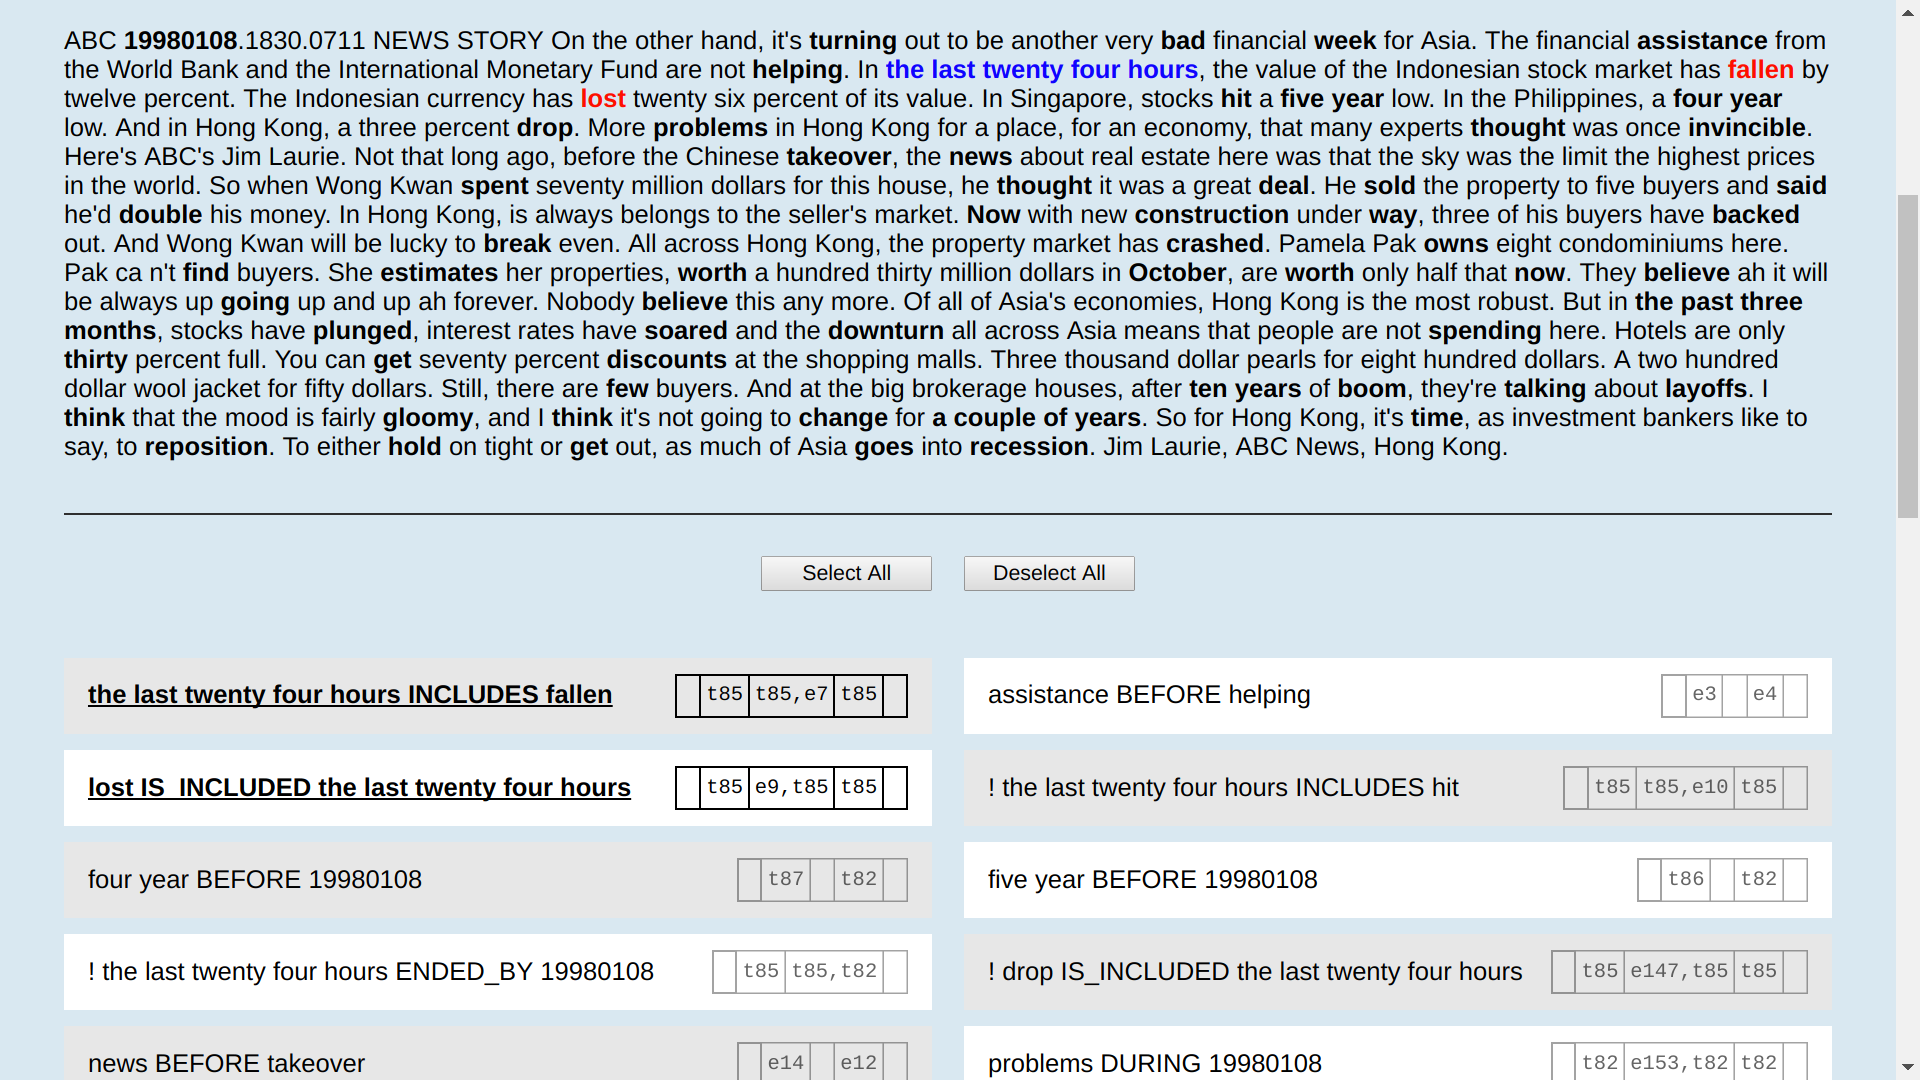
\includegraphics[width=\textwidth]{images/util1}
%	\caption{Interface for exploring the TLINKs of a TimeML document as strings.}
%	\label{figure:tlinkstrings}
%	\end{figure}
%\end{center}
%The second tool (shown in Figure \ref{figure:experimentsp}) allows a user to experiment with superposition. Strings are input either manually (by typing, for example ``\verb!|a||a'|!"), or by giving two fluent names and choosing the Allen relation between them. Hitting the return key then adds this string to a list which the user can manipulate: hovering over a string allows it to be removed from the list, or edited with some simple string operations; dragging one string onto another will superpose them and add the results to the list.
%\url{https://www.scss.tcd.ie/~dwoods/star}
%\begin{center}
%	\begin{figure}[!h]
%		\centering
%		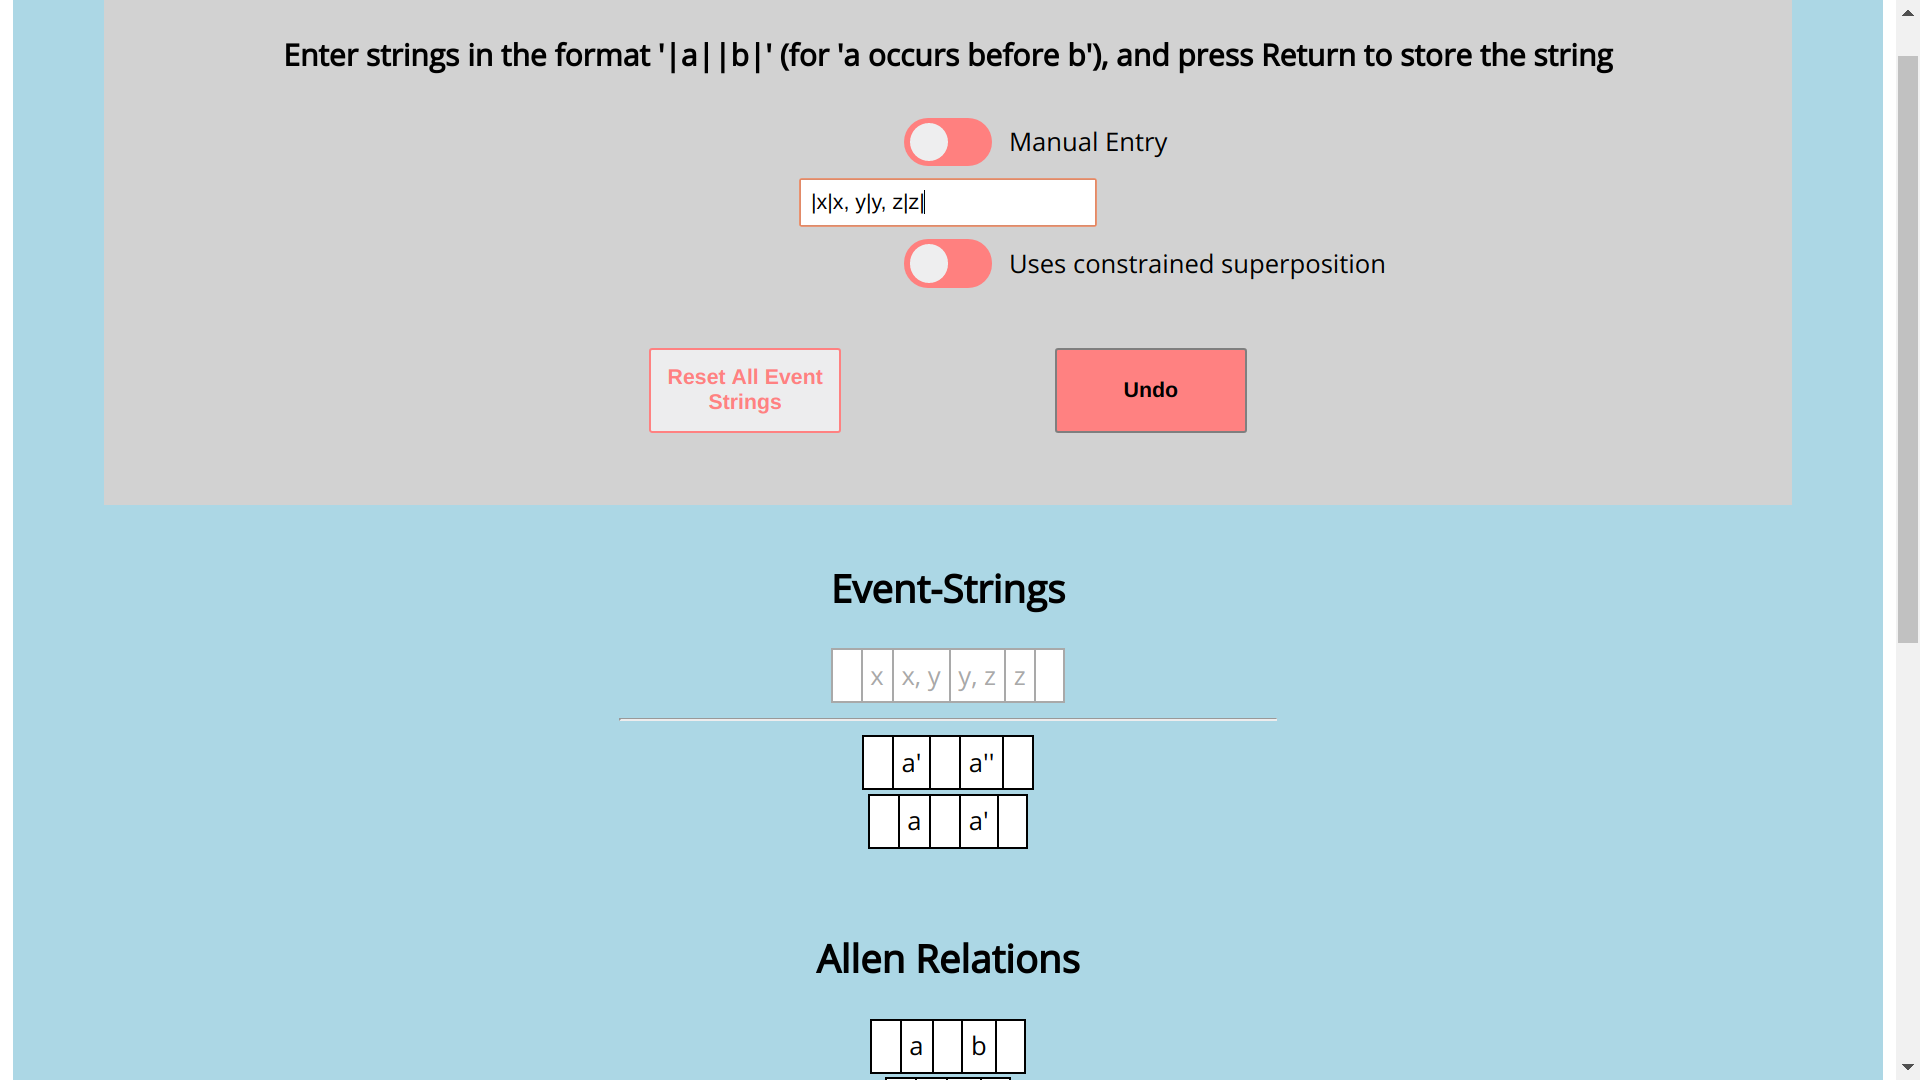
\includegraphics[width=\textwidth]{images/util2}
%		\caption{Interface for experimenting with superposition.}
%		\label{figure:experimentsp}
%	\end{figure}
%\end{center}
%One aim is for further tooling to eventually be created that might, for example, assist an annotator who is manually marking up a document with temporal relations, by displaying an updating string (or strings) which show the overall temporal structure of the document as they have annotated it so far, revealing inconsistencies, automatically computing simple transitivities, and suggesting the possibilities if superposition gives a set of more than one string. It is hoped that this kind of semi-automatic tool might be viewed as a useful complement to existing options such as T-BOX, so as to offer the annotator a greater range of representational choices.
%
%\newpage
%\section{Future Directions}\label{sec:future}
%%There are several steps still to be taken in this work. The most pressing task is currently to design an experiment which will empirically evaluate the effectiveness of strings in practice. As an anonymous reviewer commented on \citet{woods2018improving}, ``Visual appeal is in the eye of the beholder.'' The present approach should be empirically compared to alternatives (e.g. graph-based displays, T-BOX, etc.) in terms of efficiency and cognitive appeal. Documents should be created for which the complete temporal closure is available, to act as gold standard data for the experiment, as the corpus in current use, TimeBank, is generally quite far from fully annotated (and a number of the documents have inconsistencies in them \citep[p. 230]{Verhagen2005}).
%
%%While the basic framework has been put in place, such that events and times are representable using strings which can be precisely interpreted so as to determine the order and relations
%
%The work done so far, as described in Section \ref{sec:current}, has laid out the foundational elements for answering the questions posed in Section \ref{sec:intro}, but there are still several steps which must be taken. Events and times have been made representable as elements of timeline-like strings, and methods have been described for increasing data density through superposition of groups of these strings. However, the inferential power and efficiency of the strings is yet to be evaluated, and the optimal method for treatment of partial and incomplete temporal data is still untested. It is anticipated that the work will progress through the stages laid out below.
%
%\subsection{Semantic Representation}\label{sub:drs}
%
%One of the questions this work posits relates to semantic reasoning: how the strings used to represent temporal data can be used to infer logical consequences. For example, being able to determine whether one string or language entails another. Although some paths towards answering this question have already been explored in Sections \ref{sub:mso} and \ref{sub:projection}, other systems will also be examined for the purposes of comparison and evaluation of the use of strings.
%
%One of the better-known existant frameworks for semantically representing information for this kind of inference is Discourse Representation Theory (DRT), introduced by \citet{Kamp1993}. It makes use of discourse representation structures (DRSs), composed of a set of discourse referents (entities under discussion), as well as a set of DRS conditions, which describe what is known about the referents. For example, the sentence (\ref{ex:drstext}) is represented by the DRS (\ref{ex:drs}), where the top box contains the discourse referents $x$ and $y$, and the lower box contains the information about these entities:
%\begin{subequations}
%	\begin{align}
%	\onehalfspacing
%	\text{``John owns a dog."}\label{ex:drstext}\\
%	\drs{$x$~ ~$y$}{John($x$)\\[-0.5em]dog($y$)\\[-0.5em]$x$ owns $y$}\label{ex:drs}
%	\end{align}
%\end{subequations}
%DRT frequently appears as the basis for reasoning over data. For example, \citet{Bunt2015} proposed its use as the semantics behind the syntax of interoperable annotation systems; \citet{Bird2009} included modules for processing DRSs in their popular Natural Language Toolkit (NLTK) for Python; \citet{Bos2008} created a tool for creating DRSs for texts, Boxer, which is claimed to have over 95\% coverage for semantic analysis of newswire texts -- this tool in particular also features in the Parallel Meaning Bank (\url{http://pmb.let.rug.nl/}), a parallel corpus for English, German, Dutch, and Italian with semantic annotation. DRT is also capable of representing time and events, such as in (\ref{ex:drseventboth}) below:
%\begin{subequations}\label{ex:drseventboth}
%	\begin{align}
%	\onehalfspacing
%	\text{``Sarah rode the bus on Monday."}\label{ex:drseventtext}\\
%	\drs{$x$~ ~$y$~ ~$e$~ ~$t$}{Sarah($x$)\\[-0.5em]the bus($y$)\\[-0.5em]Monday($t$)\\[-0.5em]ride($e,x,y$)\\[-0.5em]Time($e,t$)}\label{ex:drsevent}
%	\end{align}
%\end{subequations}
%It will be useful to construct a translation from DRSs to strings, as this would allow for comparisons to be drawn more readily, and for evaluations to be made of the inferencing power and efficiency of the strings. There is already a translation from DRSs to First-Order Logic (described in \citet{Kamp1993}), and the performance of First-Order theorem provers (as in \citet{Bos2008}) could be compared against that of the finite-state methods for reasoning over strings. It would also be interesting to step from using just Allen's intervals to a more semantic approach to temporal data as exists in DRT. Finally, it would be informative to compare how DRT and TimeML treat the same source text, and how that may affect the strings that can ultimately be obtained as projections of both temporal annotation and DRSs to describe the document's overall temporal structure.
%
%\subsection{Incomplete Information}\label{sub:incomplete}
%
%With regards to treating incomplete information, the methods for how semi-intervals are integrated into the framework will be further developed and refined, as these appear to have potential to allow for much greater expressivity for the strings than solely using Allen's relations. However, they currently feel a little clumsy, especially when a relation is fully unconstrained: using formulae beyond just fluents within the string boxes adds a layer of complexity and seems less intuitive when reading the strings. Further, in cases where languages can't be reduced to a single string (such as the fully unconstrained relation), the current method for performing vocabulary constrained superposition is to superpose each string in the language with the other string (or each string in the other language), which can lead to a rapid increase in the size of the languages involved. Since the goal is to be working with single strings, this scenario is not ideal.
%
%In order to handle these issues, some potential avenues of progression have been identified, although their effectiveness must be thoroughly explored before being fully integrated within the framework. One option is to simply show an annotator all of the possibilities, and let them decide what to do. For example, if the five strings associated with the Freksa \textit{older} relation are produced by a superposition, the annotator could simply be shown all five. They might choose one of those five as being correct, or they might say that the \textit{older} relation is the most accurate label in that particular scenario.\footnote{Assuming that the annotator is working with TimeML, currently the only relations they can choose are from Figure \ref{table:TLINKs}, and they cannot choose disjunctions of them. A modified version, though, could allow for other relations to be chosen.} This approach, however, might not be ideal for applications other than annotation, or in fully automated systems. A second option is to use statistical methods to choose which string is the most likely; this idea is briefly discussed in \citet{woods2018improving} by looking at the relation between the fluents $c$ and $d$ in the result of the superposition \EventString{{}|a|b|{}|d|{}} $\spvc$ \Before{a}{c}, which is a language of twenty-five strings. All thirteen Allen relations appear in that language -- however, they do not appear in equal measure. Five of the strings (20\%) suggest the relation $c$ \textit{before} $d$; each of \textit{meets}, \textit{overlaps}, \textit{contains}, and \textit{finished by} appear in three strings (12\%), with the remaining eight relations appearing in just one string (4\%) each. These percentages might be used to decide (or suggest to an annotator) that \textit{before} is the most likely option. Alternatively, if Freksa relations are allowed for, 68\% of the strings in the language project to the characteristic string for $c$ \textit{older} than $d$. However, this approach does risk choosing incorrect relations just because they were more likely. This could be tested by examining how often the probabilistically chosen relation would be the same as what is given by the corpus.
%
%A further alternative could be to simply choose not to superpose strings in cases where the constraints (or lack thereof) mean that a large number of strings will be produced. Arguably, two deterministic strings are more useful than twenty-five strings which lead to non-determinism. This might result in creating a set of maximal substrings rather than one single string which acts as the timeline-like temporal structure of the document. Borrowing the example from \citet[p. 85, (35, 36)]{woods2018improving}:
%\begin{align}
%\{~ \EventString{{}|ei80|{}|t10|{}}, \EventString{{}|ei73|{}|t9|{}}, \EventString{{}|ei74|{}|ei73|{}},\notag\\ \EventString{{}|ei75|{}|ei74|{}}, \EventString{{}|ei73,ei76|{}}, \EventString{{}|ei81|ei80,ei81|{}} ~\}\label{ex:fewtlinks}\\
%\{~ \EventString{{}|ei75|{}|ei74|{}|ei73,ei76|{}|t9|{}}, \EventString{{}|ei81|ei80,ei81|{}|t10|{}} ~\}\label{ex:maximal}
%\end{align}
%where (\ref{ex:fewtlinks}) is a very small document from TimeBank,\footnote{Document wsj\_0006.tml} with the TLINKs converted to strings. (\ref{ex:maximal}) is the result of superposing all of the strings in (\ref{ex:fewtlinks}) together until there are no more options which lead to single-string languages. These two resulting strings have no fluents in common, so superposing them together wouldn't provide any new information, and the maximal substrings for the document have been found. This gives two disjoint but deterministic timelines for the document, as opposed to a non-deterministic set of possible timelines. Again, whether this approach is useful or not may depend on the application: a human annotator might prefer determinism, while an automated system might find the non-deterministic approach more feasible for use. An algorithm to reduce a TimeML document to its set of minimal substrings was run on each file in the TimeBank corpus, which found (while highlighting 17 documents with inconsistencies) a total of 7852 events and 6393 TLINKs were reduced to 3190 timeline strings, a reduction of just over 59\% or 50\% depending on whether one considers the events or their relations as the more salient metric to be reduced.
%
%Additionally, \citet{van1996design} discuss some heuristics and techniques for improving the efficiency of temporal reasoning algorithms, including for composition of relations and consistency-checking. These techniques are not currently implemented in the present work, but their applicability to the strings will be explored, as they may lead to improvements in the speed of calculating superposition in large strings which contain large numbers of fluents.
%
%%Following the direction of \citet{Fernando2018}, the framework will continue to be fleshed out such that it might handle both intervals and points at the same time, as well as introducing of the concept of opposable forces -- i.e. forces which will effect a change to some fluent(s) in a string. For example, currently the framework might have the following string \Meets{do}{ds}, with $do = \text{``Door is open"}$, $ds = \overline{do} = \text{``Door is shut"}$, modelling the scenario that a door was open one moment, then closed in the next. A force $cd = \text{``Close the door''}$ could be described which causes an open door to become closed and update the string to be \Meets{do, cd(do)}{ds}, which says that the door is open in the first moment, and simultaneously a force is applied which will cause the door to be closed in the next moment. By ``opposable'' forces, it is understood that another force $od = \overline{cd} = \text{``Open the door''}$ could exist which is the negation of $cd$. If both forces are applied in the same moment, they will oppose each other and cancel out.
%
%\subsection{Applications}\label{sub:applications}
%
%Further to the utilities described in Section \ref{sub:implementation}, tooling for experimentation and evaluation is to be developed which will allow for testing aspects such as the probabilistic reasoning, and for comparison of the various approaches described above for treating and reasoning about incomplete information. Existing tools such as Boxer \citep{Bos2008} and NLTK \citep{Bird2009} will be integrated into the workflow in order to experiment with DRT and evaluate the semantic aspects of the framework.
%
%While developing larger applications to use the strings is outside of the scope of this work, it is anticipated that the most eminent use would be as tooling such that an annotation environment might implement in a complementary fashion, alongside established tools like Tango and T-BOX. The goal would be to allow the annotator to switch freely between this and other representations so that they may use whichever style seems to suit them best, hopefully enabling them to produce higher quality annotations. Other possible applications for the strings might include the automatic summarisation\footnote{Some work in this direction: \citet{Yan2011}} and/or aggregation of documents based on their timelines, or in a similar vein, automatic corroboration of details between different accounts of the same events, or checking the veridicality of reported speech against actual events, using timelines as the basis for comparison.



%%%%%%%%%%%%%%%%%%%%%%%%%%%%%%%%%%%%%%%%%%%%%%%%%%%%%%%%%%%%%%%%%%%%%%%%%%%%%%%%
%                                                                              %
%                             Actual Document Ends                             %
%                                                                              %
%%%%%%%%%%%%%%%%%%%%%%%%%%%%%%%%%%%%%%%%%%%%%%%%%%%%%%%%%%%%%%%%%%%%%%%%%%%%%%%%
\newpage
\pagestyle{empty}
\onehalfspacing
\bibliographystyle{apa}
\bibliography{refs}
\end{document}